% This is the main file for the template for doctoral thesis at
% University of Zagreb, Faculty of Electrical Engineering and Computing
% in Zagreb, Croatia.
% Initial version was created in April 2013, last update was in July 2014.

% Author: Jelena Bozek, jelena.bozek@fer.hr
% Contributor: Vedran Miletic, vmiletic@inf.uniri.hr


%%%%%%%%%%%%%%%%%%%%%%%%% POSTAVKE / SETTINGS %%%%%%%%%%%%%%%%%%%%%%%%%%%%%
\documentclass[12pt,oneside, a4paper]{book}
\usepackage{etex}
\usepackage{xcolor}
\usepackage[pdftex]{graphicx}
\usepackage{rotating}
\usepackage{epsfig}
\usepackage{epstopdf}
% required for printing index
% use \index{name} in text
%\usepackage{makeidx}
%\makeindex
% required for printing nomenclature
% use \nomenclature{symbol}{description} in text
%\usepackage{nomencl}
%\makenomenclature
%\renewcommand{\nomname}{Popis oznaka}

\usepackage[T1]{fontenc}
\usepackage[utf8]{inputenc}
\usepackage{cmap}
%\usepackage[croatian]{babel}
\usepackage{ae}
\usepackage[unicode]{hyperref}
\usepackage{mathptmx}
\usepackage{amscd}
\usepackage{amssymb}
\usepackage{amsmath}
\usepackage{amsfonts}

\usepackage[left=2.5cm,right=2.5cm,top=2.5cm,bottom=2.5cm]{geometry}
\usepackage{setspace} 
\linespread{1.3}
\usepackage{fancyhdr} % setting up header and position of page numbers
\pagestyle{fancyplain}
\fancyhf{}
\lhead{\nouppercase{\fancyplain{}{\leftmark}}}
\renewcommand{\chaptermark}[1]{\markboth{#1}{}}
\rfoot{\thepage}

\usepackage{hhline}
\usepackage{enumerate}
\usepackage{delarray}
\usepackage{array}  % package for some table properties
\usepackage{tabularx} % package that allows dynamical changing table cell width
\usepackage{multirow}  % package that enables multiple rows in a table
\usepackage[bf, font=small]{caption}
\usepackage[labelfont=small, font=small]{subcaption}
\usepackage{wasysym}
\usepackage{subeqnarray}
\usepackage{aeguill}
\usepackage{pdflscape} % setting page into landscape view
\usepackage{enumitem} % for itemize lists
\setlist{nolistsep}   % setting for itemize lists

\renewcommand{\thefootnote}{\fnsymbol{footnote}}  % to get unnumbered footnotes
\renewcommand{\arraystretch}{1.5} % stretching row height

\usepackage[square, numbers, sort]{natbib} 



% Adding a dot after chapter number in TOC 
\let\savenumberline\numberline
\def\numberline#1{\savenumberline{#1.}}

% Adding dots after chapter titles to page number in TOC
\makeatletter
\renewcommand*\l@chapter[2]{%
  \ifnum \c@tocdepth >\m@ne
  \addpenalty{-\@highpenalty}%
  \vskip 1.0em \@plus\p@
  \setlength\@tempdima{1.5em}%
  \begingroup
  \parindent \z@ \rightskip \@pnumwidth
  \parfillskip -\@pnumwidth
  \leavevmode \bfseries
  \advance\leftskip\@tempdima
  \hskip -\leftskip
  #1\nobreak\normalfont\leaders\hbox{$\m@th
    \mkern \@dotsep mu\hbox{.}\mkern \@dotsep
    mu$}\hfill\nobreak\hb@xt@\@pnumwidth{\hss #2}\par
  \penalty\@highpenalty
  \endgroup
  \fi}
\makeatother

% adjust the line spacing in a matrix
\makeatletter
\renewcommand*\env@matrix[1][\arraystretch]{%
  \edef\arraystretch{#1}%
  \hskip -\arraycolsep
  \let\@ifnextchar\new@ifnextchar
  \array{*\c@MaxMatrixCols c}}
\makeatother

% remove footer (page number) from TOC, list of figures and list of tables
\AtBeginDocument{\addtocontents{toc}{\protect\thispagestyle{empty}}}
\AtBeginDocument{\addtocontents{lof}{\protect\thispagestyle{empty}}}
\AtBeginDocument{\addtocontents{lot}{\protect\thispagestyle{empty}}}


\begin{document}


%%%%%%%%%%%%%%%%%%%%%%%%%%%%%%%%%%%%%%%%%%%%%%%%%%%%%%%%%%%%%%%%%%%%%%%%%%%
\frontmatter

%%%%%%%%%%%%%%%%%%%% NASLOVNICA / FRONT COVER PAGE %%%%%%%%%%%%%%%%%%%%%%%%
\begin{titlepage}
  \fontsize{16pt}{20pt}\selectfont
  \fontfamily{phv}\fontseries{mc}\selectfont
  \newgeometry{left=3cm,right=3cm,top=3cm,bottom=2.5cm}
  \setlength{\intextsep}{0pt plus 0pt minus 0pt}

  \begin{center}
    \begin{figure}[ht!]
      \begin{center}
        
\includegraphics[height=4.1184cm, width=5.94cm]{logo_unizg_eng}
      \end{center}
    \end{figure}
    \vspace{0cm}
    {FACULTY OF SCIENCE} \\
    \vspace{3cm}
    Jelena Luetić \\
    \vspace{2cm}
    {\fontsize{22pt}{22pt}\selectfont\textbf{Measurement of the cross section for associated production of a W boson and two b quarks with the CMS detector at the Large Hadron Collider}} \\
    \vspace{2cm}  
    DOKTORSKI RAD \\    
    \vfill{Zagreb, 2015.}
  \end{center}
  \restoregeometry
\end{titlepage}
%%%%%%%%%%%%%% Prva UNUTARNJA STRANICA / SECOND INNER PAGE %%%%%%%%%%%%%%%
\begin{titlepage}
  \fontsize{16pt}{20pt}\selectfont
  \fontfamily{phv}\fontseries{mc}\selectfont
  \newgeometry{left=3cm,right=3cm,top=3cm,bottom=2.5cm}
  \setlength{\intextsep}{0pt plus 0pt minus 0pt}

  \begin{center}
    \begin{figure}[ht!]
      \begin{center}
        
\includegraphics[height=4.1184cm, width=5.94cm]{logo_unizg_eng}
      \end{center}
    \end{figure}		
    \vspace{0cm}
    {\fontsize{16pt}{16pt}{FACULTY OF SCIENCE}} \\
    \vspace{3cm}
    Jelena Luetić \\
    \vspace{2cm}
    {\fontsize{22pt}{22pt}\selectfont\textbf{Measurement of the cross section for associated production of a W boson and two b quarks with the CMS detector at the Large Hadron Collider}} \\
    \vspace{2cm}   
    DOCTORAL THESIS \\  
    \vspace{5cm}   % adjust this spacing if necessary
    Supervisor: Professor Vuko Brigljević, PhD \\
    \vfill{Zagreb, 2015}
  \end{center}
  \restoregeometry
\end{titlepage}
%%%%%%%%%%%%%%% Druga UNUTARNJA STRANICA / FIRST INNER PAGE %%%%%%%%%%%%%%%%
\begin{titlepage}
  \fontsize{16pt}{20pt}\selectfont
  \fontfamily{phv}\fontseries{mc}\selectfont
  \newgeometry{left=3cm,right=3cm,top=3cm,bottom=2.5cm}
  \setlength{\intextsep}{0pt plus 0pt minus 0pt}

  \begin{center}
    \begin{figure}[ht!]
      \begin{center}
        
\includegraphics[height=4.1184cm, width=5.94cm]{logo_unizg2}
      \end{center}
    \end{figure}		
    \vspace{0cm}
    {PRIRODOSLOVNO MATEMATIČKI FAKULTET} \\
    \vspace{3cm}
    Jelena Luetić \\
    \vspace{2cm}
    {\fontsize{22pt}{22pt}\selectfont\textbf{Mjerenje udarnog presjeka zajedničke produkcije W bozona i para b kvarkova CMS detektorom na Velikom hadronskom sudarivaču}} \\
    \vspace{2cm}    
    DOKTORSKI RAD \\
    \vspace{5cm}    % adjust this spacing if necessary
    Mentor: Prof. dr. sc. Vuko Brigljević \\
    \vfill{Zagreb, 2015.}
  \end{center}
  \restoregeometry
\end{titlepage}



%%%%%%%%%%%%%%%%%%%%%%%%%%%%%%%%%%%%%%%%%%%%%%%%%%%%%%%%%%%%%%%%%%%%%%%%%%%
\begin{titlepage}
  \begin{minipage}{\dimexpr\textwidth-1cm}
    \vspace{3cm}
    Doktorski rad izrađen je na Sveučilištu u Zagrebu
    Prirodoslovno matematičkom fakultetu

    \vspace{1cm}
    Mentor: prof. dr. sc. Vuko Brigljević

    \vspace{1cm}
    Doktorski rad ima: XYZ stranica

    \vspace{1cm}
    Doktorski rad br.: \line(1,0){64}
  \end{minipage}
\end{titlepage}


%%%%%%%%%%%%%%%%%%%%%%%%%%%%%%%%%%%%%%%%%%%%%%%%%%%%%%%%%%%%%%%%%%%%%%%%%%%
% insert optional page with thanks or dedication
%\include{eg_thanks_dedication}



%%%%%%%%%%%%%%%%%%%%%%%%%%%%%%%%%%%%%%%%%%%%%%%%%%%%%%%%%%%%%%%%%%%%%%%%%%%
\clearpage
%%%%%%%%%%%%%%%%%%%%%%%%%%%%%%%%% TOC %%%%%%%%%%%%%%%%%%%%%%%%%%%%%%%%%%%%%
\pagestyle{empty} % remove header/footer 
\tableofcontents
\cleardoublepage % start new page

%\pagestyle{fancyplain} % puts headers/footers back on


%%%%%%%%%%%%%%%%%%%%%%%%%%%%%%%%%%%%%%%%%%%%%%%%%%%%%%%%%%%%%%%%%%%%%%%%%%%

\mainmatter % Begin numeric (1,2,3...) page numbering

\pagestyle{fancy} % Return the page headers back to the "fancy" style

% Include the chapters of the thesis as separate files from the Chapters folder
% Uncomment the lines as you write the chapters

%% Chapter 1

\chapter{Introduction} % Main chapter title

\label{Chapter1} % For referencing the chapter elsewhere, use \ref{Chapter1} 

\lhead{Chapter 1. \emph{Introduction}} % This is for the header on each page - perhaps a shortened title

% Filozofija
The standard model of particle physics tries to give an answer to the questions what is the matter made of and how does it interact. The predictions of the standard model have been thoroughly tested many times and various precision measurements were performed at different experiments. Nevertheless every time the standard model predictions were confirmed. The only missing link, the long sought Higgs boson, was found in 2012, with its properties measured in the following years thus completing the picture of elementary particles. However, standard model still leaves some unexplained phenomena, e.g. neutrino oscillations, matter-antimatter asymmetry, the existence of dark matter and dark energy, giving rise to the physics beyond standard model. The sensitivity of such processes in the high energy physics experiments strongly depends on the precise measurements of known processes. In such measurements, poorly known yields and kinematics of the known processes would lead to high uncertainties, and thus reducing the sensitivity of the experiment. 
% Zasto b kvark - QCD
\par The production of a W boson in association with a pair of b quarks (Wbb) has
been the topic of many theoretical studies and simulations. It is however still not well described due to collinear and infrared divergences. Several theoretical
approaches, implemented in different simulation packages, have been used to describe the Wbb production mechanism. A precise measurement of Wbb production will allow to
further constrain theoretical predictions in the framework of perturbative quantum chromodynamics (pQCD) and to test the validity of different theoretical models used in simulations. On the other hand, Wbb is a background to different standard model processes as well as beyond standard model searches. It is one of the main backgrounds to top quark  and Higgs boson measurements, in particular, events in which Higgs boson is produced in association with a W boson and decays to a pair of b quarks.
% Sto je pokazano
\par This thesis is focused on the measurement of the cross section of $pp\rightarrow W+bb+X$ process using the data collected during 2012 at $\sqrt{s} = 8$ TeV. W boson is decaying either to an electron or muon, and a corresponding neutrino. The presence of a W boson is identified through the detection of an energetic, isolated lepton, i.e. lepton without any additional activity in some predefined cone around it, and a significant amount of missing energy, which indicates the presence of a neutrino. Jets in the detector are identified as a collimated spray of particles. Selected jets are required to be tagged as jets originating from b quarks. This procedure is called b-tagging and it exploits unique b quark properties to derive a single discriminator value to distinguish between b jets and jets from lighter quarks, or gluons. 
% Organizacija teze

The thesis is organized as follows. Chapter 2 shows a brief introduction to the standard model, with the emphasis on the discovery and the role of W boson and b quarks within the standard model. An overview of the phenomenology of the proton collisions at hadron colliders is shown. Steps for the theoretical calculation of the $pp\rightarrow W+bb+X$ process are given for both, single parton scattering and double parton scattering production mechanisms. The end of the chapter summarizes all previous measurements of W boson and b quarks in the final state. Chapters 3 and 4 are focused on the description of the LHC and CMS respectively. All CMS subsystems are described and their role is explained. Chapter 5 describes the procedure for reconstruction of various physics objects, including electrons, muons and jets, and estimation of missing energy. Chapter 6 lists all data and Monte Carlo samples used. Criteria for the signal selection is described and all major backgrounds are identified. Chapter 7 describes all steps in the cross section determination, including the fitting procedure used to extract final yields, and the acceptance and efficiency estimation. In the end, the results are presented, together with the comparison to theoretical predictions. Final chapter briefly summarizes the results, and shows the prospects for the future research on this topic.

% Chapter Template

\chapter{Standard Model} % Main chapter title

\label{Chapter2} % Change X to a consecutive number; for referencing this chapter elsewhere, use \ref{ChapterX}

\lhead{Chapter X. \emph{Chapter Title Here}} % Change X to a consecutive number; this is for the header on each page - perhaps a shortened title

%----------------------------------------------------------------------------------------
%	SECTION 1
%----------------------------------------------------------------------------------------

\section{Standard model}

Lorem ipsum dolor sit amet, consectetur adipiscing elit. Aliquam ultricies lacinia euismod. Nam tempus risus in dolor rhoncus in interdum enim tincidunt. Donec vel nunc neque. In condimentum ullamcorper quam non consequat. Fusce sagittis tempor feugiat. Fusce magna erat, molestie eu convallis ut, tempus sed arcu. Quisque molestie, ante a tincidunt ullamcorper, sapien enim dignissim lacus, in semper nibh erat lobortis purus. Integer dapibus ligula ac risus convallis pellentesque.

%-----------------------------------
%	SUBSECTION 1
%-----------------------------------
\subsection{Wbb at hadron collider}

Nunc posuere quam at lectus tristique eu ultrices augue venenatis. Vestibulum ante ipsum primis in faucibus orci luctus et ultrices posuere cubilia Curae; Aliquam erat volutpat. Vivamus sodales tortor eget quam adipiscing in vulputate ante ullamcorper. Sed eros ante, lacinia et sollicitudin et, aliquam sit amet augue. In hac habitasse platea dictumst.

%-----------------------------------
%	SUBSECTION 2
%-----------------------------------

\subsection{Previous measurements}
Morbi rutrum odio eget arcu adipiscing sodales. Aenean et purus a est pulvinar pellentesque. Cras in elit neque, quis varius elit. Phasellus fringilla, nibh eu tempus venenatis, dolor elit posuere quam, quis adipiscing urna leo nec orci. Sed nec nulla auctor odio aliquet consequat. Ut nec nulla in ante ullamcorper aliquam at sed dolor. Phasellus fermentum magna in augue gravida cursus. Cras sed pretium lorem. Pellentesque eget ornare odio. Proin accumsan, massa viverra cursus pharetra, ipsum nisi lobortis velit, a malesuada dolor lorem eu neque.

%----------------------------------------------------------------------------------------
%	SECTION 2
%----------------------------------------------------------------------------------------

\section{Main Section 2}

Sed ullamcorper quam eu nisl interdum at interdum enim egestas. Aliquam placerat justo sed lectus lobortis ut porta nisl porttitor. Vestibulum mi dolor, lacinia molestie gravida at, tempus vitae ligula. Donec eget quam sapien, in viverra eros. Donec pellentesque justo a massa fringilla non vestibulum metus vestibulum. Vestibulum in orci quis felis tempor lacinia. Vivamus ornare ultrices facilisis. Ut hendrerit volutpat vulputate. Morbi condimentum venenatis augue, id porta ipsum vulputate in. Curabitur luctus tempus justo. Vestibulum risus lectus, adipiscing nec condimentum quis, condimentum nec nisl. Aliquam dictum sagittis velit sed iaculis. Morbi tristique augue sit amet nulla pulvinar id facilisis ligula mollis. Nam elit libero, tincidunt ut aliquam at, molestie in quam. Aenean rhoncus vehicula hendrerit. 
% Chapter Template

\chapter{Large Hadron Collider} % Main chapter title

\label{Chapter3} % Change X to a consecutive number; for referencing this chapter elsewhere, use \ref{ChapterX}

\lhead{Chapter 3. \emph{Large Hadron Collider}} % Change X to a consecutive number; this is for the header on each page - perhaps a shortened title

CERN is the largest particle physics laboratory in the world, located near the city of Genava, on the French-Swiss border. It was founded in 1953 by 12 countries and today it has 21 member states. It's main function is to provide particle accelerators and infrastructure for high energy physics experiments. Current accelerator complex is a chain of smaller accelerators with increasingly higher energies of which the largest one is Large Hadron Collider (LHC) (Figure \ref{LHC}). Protons accelerated in the chain are obtained by taking hydrogen atoms and stripping them of the orbiting electrons. Protons are then accelerated by a small linear accelerator Linac2 to 50 MeV and injected to PS Booster. After reaching 1.4 GeV, protons are injected to Proton Synchrotron and accelerated to 25 GeV. Next accelerators in chain are Super Proton Synchrotron (SPS) with energy of 450 GeV, and Large Hadron collider with beam energy of 7 TeV. 
Some of the major physics results at CERN include the discovery of neutral currents, discovery of W and Z bosons, creation of antihydrogen atom and direct observation of CP violation among others. 
In this chapter, we will briefly go through the motivation for the LHC design, building blocks of the LHC will be presented together with the accelerator performance during the past few years.   
\begin{figure}[htbp]
	\centering
		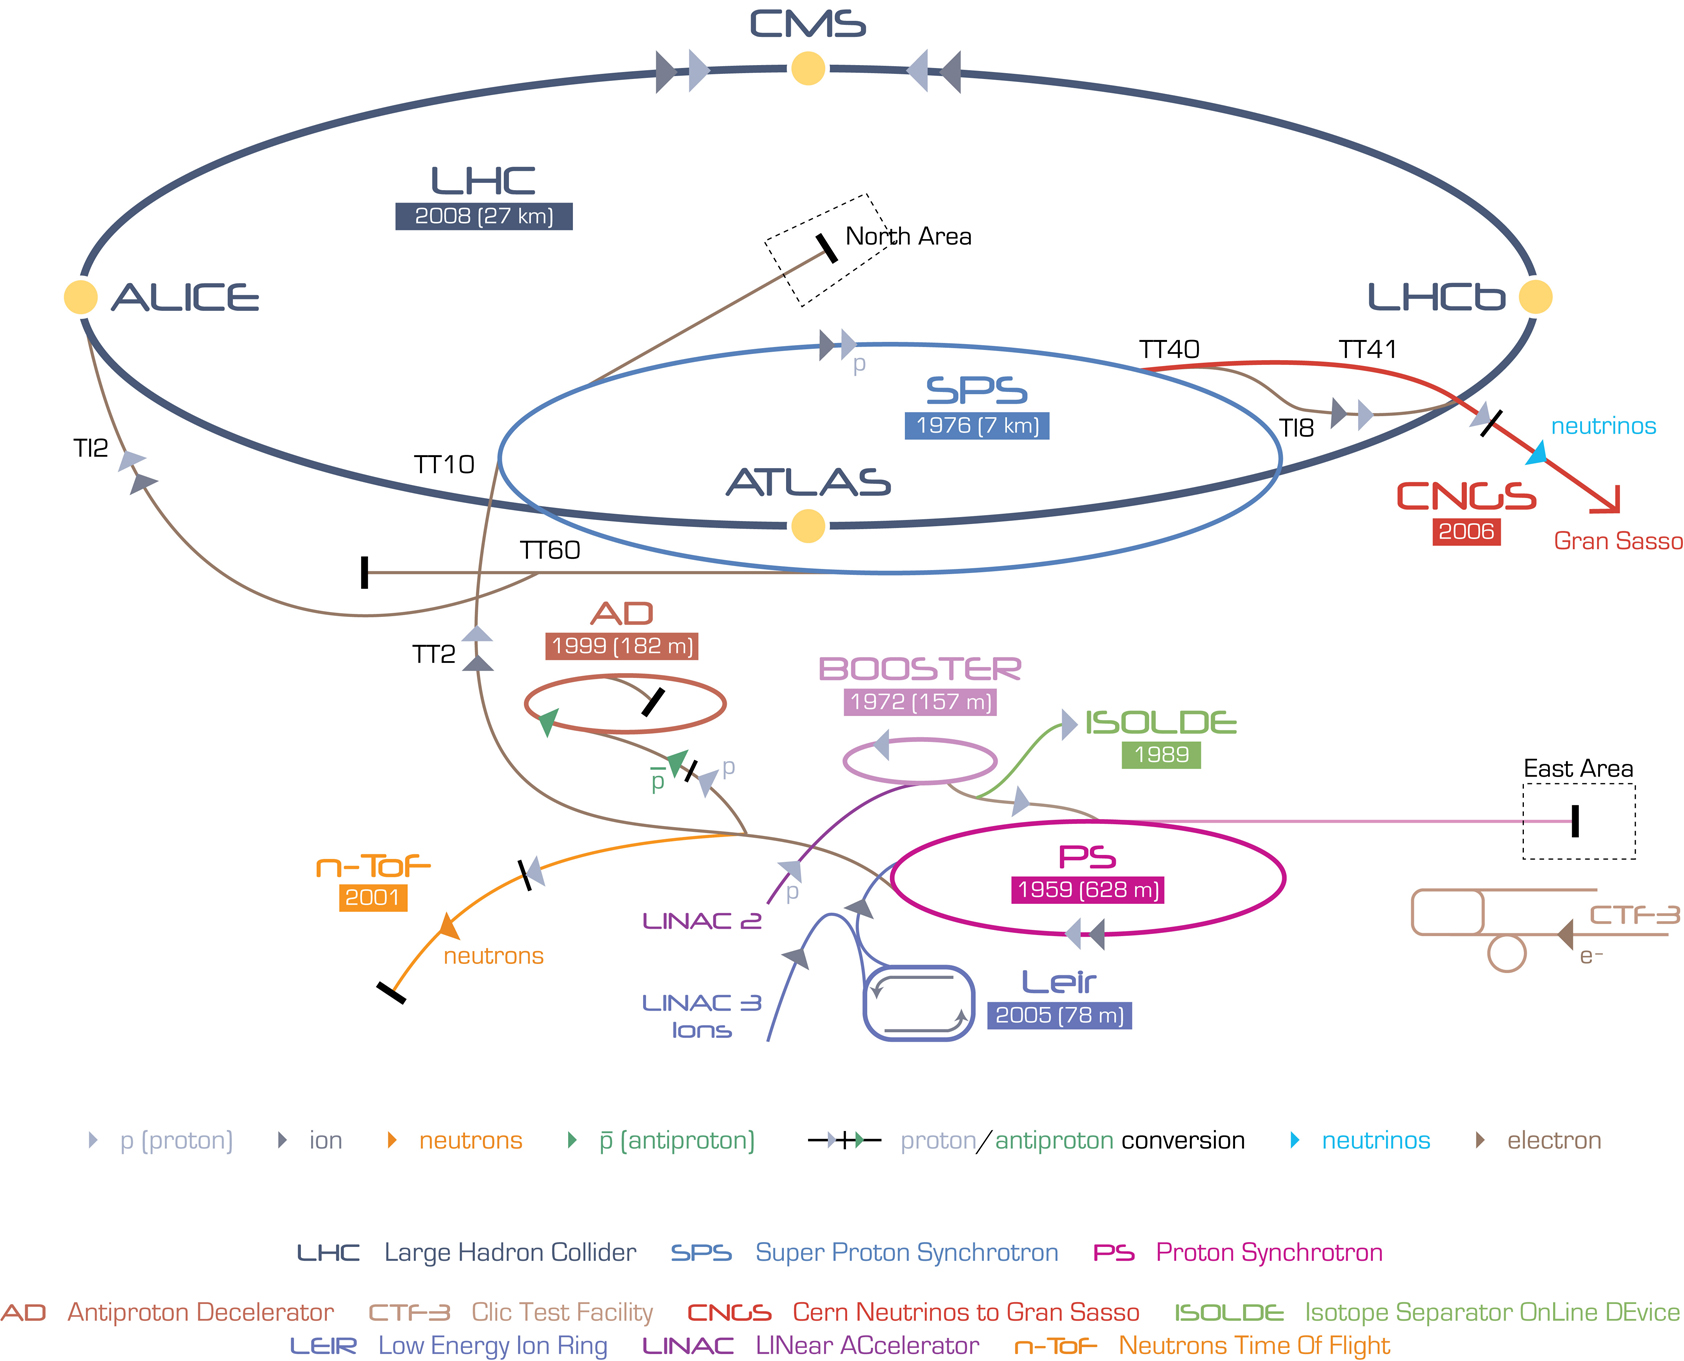
\includegraphics[width=0.8\textwidth]{Figures/LHC.jpg}
		%\rule{35em}{0.5pt}
	\caption[Schematics of Large Hadron Collider]{Schematics of Large Hadron Collider}
	\label{fig:LHC}
\end{figure}
%----------------------------------------------------------------------------------------
%	SECTION 1
%----------------------------------------------------------------------------------------

\section{Design of the Large Hadron Collider}

The Standard model of elementary particles describes nicely all known particles and interactions, however there are still some unanswered questions. One of the major question was the existence of Higgs boson which was solved in the past few years with the discovery of a new particle at 125 GeV. Other questions that is still open is the unification of fundamental forces, as it is difficult to construct a theory of gravity which would be similar to those of other fundamental interactions. One attempt to achieve this goal is the theory of supersymmetry which predicts that each particle has its heavier supersymetric partner which according to some theories could unify all fundamental forces. If the theory of supersymetry is correct, lightest supersymetic particles could be found at the LHC.  



\begin{figure}[htbp]
	\centering
		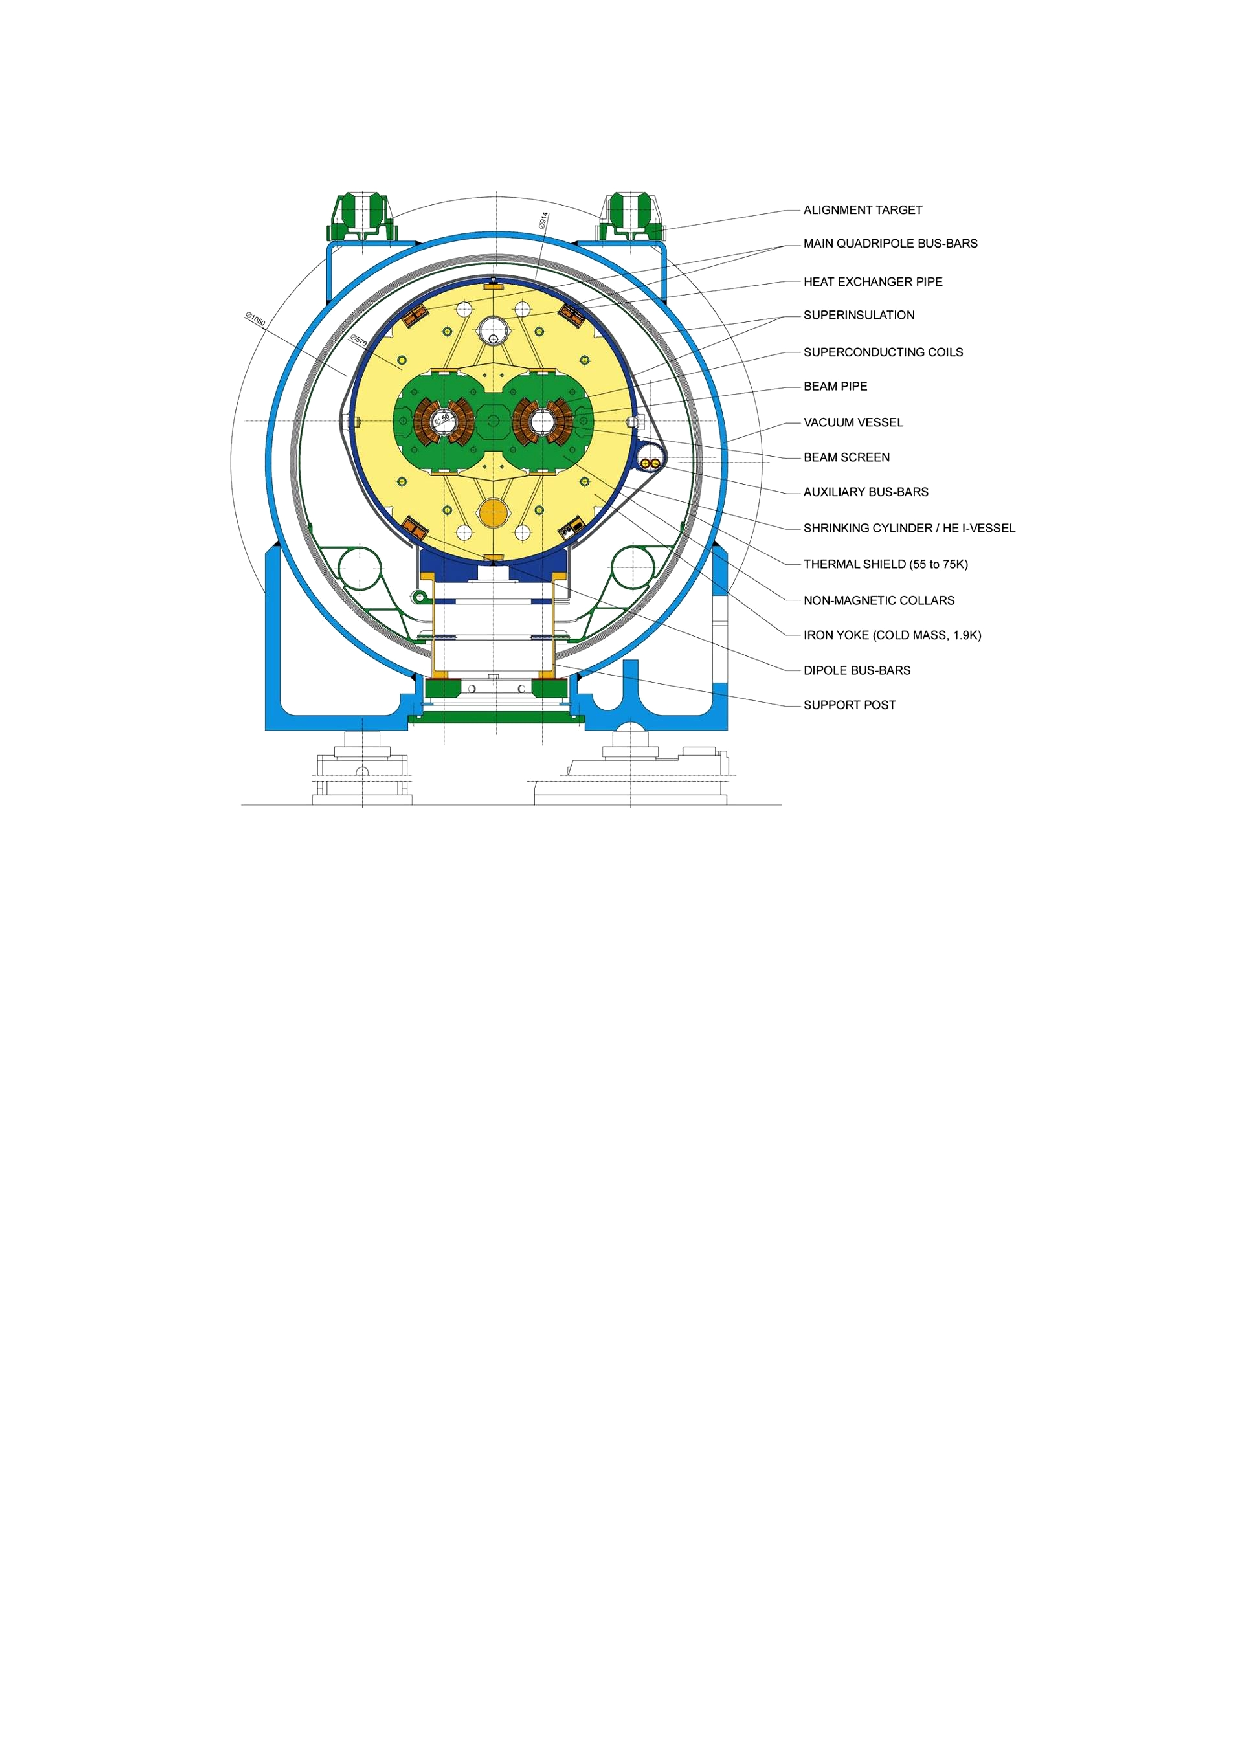
\includegraphics[width=0.7\textwidth]{Figures/LHC_magnet.pdf}
		%\rule{35em}{0.5pt}
	\caption[Schematics of dipole magnets]{Schematics of Dipole magnets}
	\label{fig:LHC_mag}
\end{figure}

%-----------------------------------
%	SECTION 2
%-----------------------------------

\section{Performance}

Since the start of the LHC in 2009, there were three years of machine operation, which yielded many physics results among which the discovery of Higgs boson reported by ATLAS and CMS collaborations. should be highlighted. First year of operation was devoted to commissioning and understanding machine characteristics with the emphasis on safety and testing machine protection systems. In 2011 new energy and instantaneous luminosity records were reached. These numbers were increased once again in 2012 with center of mass energy going to 8 TeV.
\par High bunch intensity with 50 ns bunch spacing was used in order to get a good instantaneous luminosity performance. This came at a cost of high number of collisions in one bunch crossing (pile-up) which was in 2012 around 12 collisions, and in some cases this number went as high as 20 interactions. With the increase of instantaneous luminosity in 2012, number of pile-up interactions was on the average around 30. Besides proton-proton collisions, LHC successfully delivered lead-lead ion runs in 2010 and 2011. primarily for the ALICE experiment, but also for CMS and ATLAS. At the start of 2013. there was also a successful proton-lead run performed for the first time. 

\begin{table}[h]
\centering
  \caption{LHC performance in 2012}
  \begin{tabular}{ l  c  c }
      \hline
      \hline
      Parameter & Design value & Value in 2012 \\
      \hline
      Beam energy [TeV] & 7 & 4 \\
      Bunch spacing [ns] & 25 & 50 \\
      Number of bunches & 2808 & 1374 \\
      Protons per bunch & 1.15$\times 10^{11}$ & 1.6-1.7$\times 10^{11}$ \\
      Peak luminosity [cm$^{-2}$s$^{-1}$] & 1$\times 10^{34}$ & 7.7$\times 10^{33}$ \\
      Max. number of events per bunch crossing & 19 & $\approx 40$ \\
      Stored beam energy [MJ] & 362 & $\approx$ 140 \\
      \hline
      \hline 
  \end{tabular}
\end{table}

LHC head achieved very good luminosity performance during pat years mainly because of the excellent beam quality delivered by the injectors with significantly more protons than nominal and with lower emittances. Since the LHC was capable to absorb these beams, it was chosen to continue to operate with 50 ns bunch spacing. This meant higher pile-up which had to be dealt with by the experiments. 


\begin{table}[h]
\centering
  \caption{LHC performance highlights}
  \begin{tabular}{ l  c }
      \hline
      \hline
      Max. luminosity delivered in one fill & 237 pb$^{-1}$  \\
      Max. luminosity delivered in 7 days & 1.35 fb$^{-1}$  \\
      Longest time in stable beams (2012) & 22.8 hours \\
      Longest time in stable beams over 7 days & 91.8 hours (55$\%$) \\
      \hline
      \hline 
  \end{tabular}
\end{table}

\begin{figure}[htbp]
	\centering
		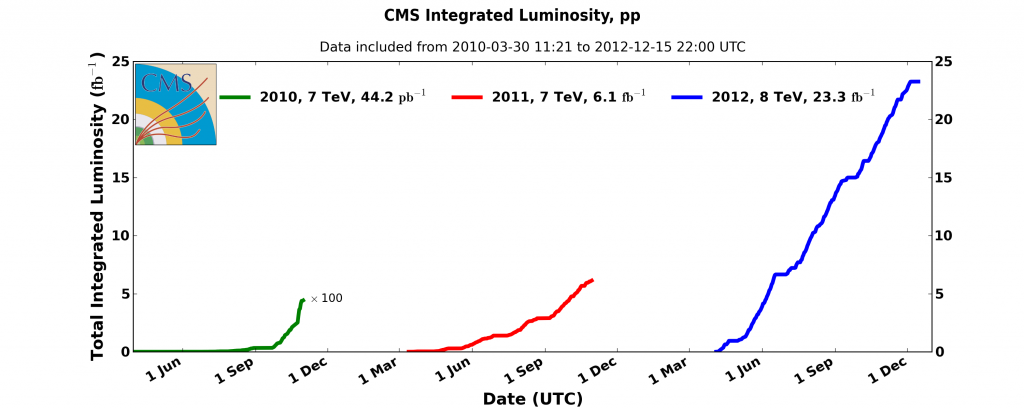
\includegraphics[width=0.7\textwidth]{Figures/lumi.png}
		%\rule{35em}{0.5pt}
	\caption[Luminosity delivered to the CMS experiment]{Luminosity delivered to the CMS experiment}
	\label{fig:LHC_lumi}
\end{figure}
 
Following a two year shutdown, LHC is anticipating operations at even higher energies of 6.5 TeV and later 7 TeV. The long term plan includes even higher peak luminosities, installation of the new injector complex and later the beginning of HL-LHC era. The timeline will, of course, be highly affected by the performance and results of the next run.
\chapter{The Compact muon solenoid} % Main chapter title

\label{Chapter4} % Change X to a consecutive number; for referencing this chapter elsewhere, use \ref{ChapterX}

\fancyhead[LE,RO]{Chapter 4. \emph{Compact Muon Solenoid}} % Change X to a consecutive number; this is for the header on each page - perhaps a shortened title

The Compact Muon Solenoid (CMS) is a general purpose detector designed to cover a wide range of physics topics at the LHC with a layered design approach and coverage of a large portion of the solid angle around the interaction point. The tracking system and calorimeters are placed inside a large soleonid in order to improve the resolution of the momentum and energy measurements. The detector outside the solenoid is aimed primarily to detection of muons. A drawing of the CMS detector is shown in Figure \ref{fig:CMS}. 
\begin{figure}[htbp]
	\centering
		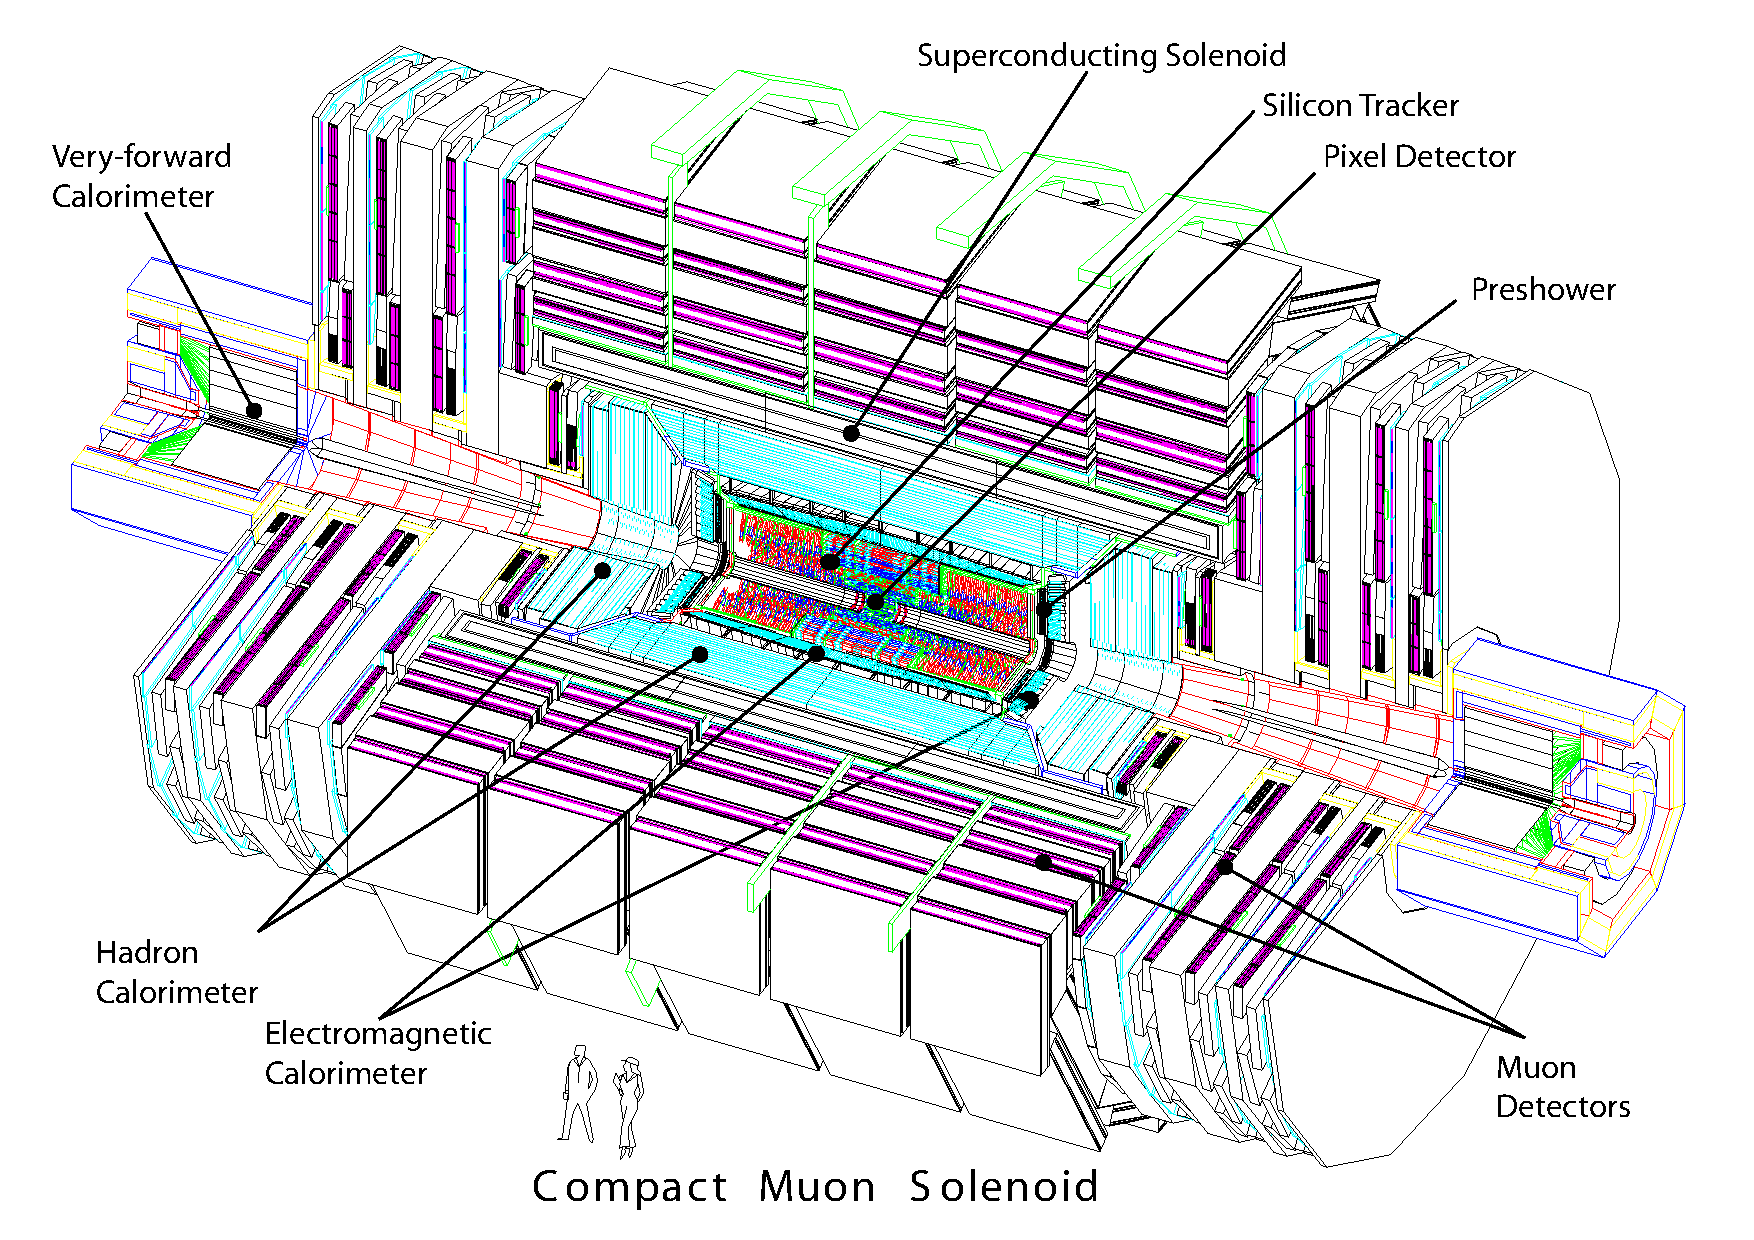
\includegraphics[width=0.9\textwidth]{Figures/CMS.pdf}
		%\rule{35em}{0.5pt}
	\caption[CMS detector]{A drawing of the CMS detector. \cite{Chatrchyan:2008aa}}
	\label{fig:CMS}
\end{figure}
\par The motivation for the CMS design with respect to its purpose in the LHC program is a very good muon identification and good momentum resolution over wide range of phase space and unambiguous determination of muon charge. Very good inner tracking system allows for detection of charged particles and high efficiency offline b quark and $\tau$ tagging. Other important requirements, specially for Higgs searches, is diphoton mass resolution, and photon and electron identification and isolation at high energies. 
CMS detector with its design meets all these requirements as is shown in following sections of this chapter. 

%----------------------------------------------------------------------------------------
%	SECTION 0
%----------------------------------------------------------------------------------------

\section{CMS coordinate system}

CMS uses a right-handed coordinate system with the origin in the nominal interaction point. $z-$axis is pointing along the beam line. $x-$axis is pointing towards the center of the LHC ring while y-axis points upwards. Two angles are used to describe position inside the detector, azimuthal angle $\phi$ and polar angle $\theta$. $\phi$ angle lies in $x-y$ plane with a range $[-\pi,\pi]$  and is defined as $\phi=$arctan$(y/x)$. The other angle $\theta$ is usually not used in high-energy physics because differences in $\theta$ are not Lorentz invariant.
The variable that is Lorentz invariant is rapidity:
\begin{equation}
y=\frac{1}{2}ln\left[ \frac{E+p_z}{E-p_z}\right]
\end{equation}
In high energy experiments in the relativistic limit where $E>>m$, a quantity called pseudorapidity is a good approximation of rapidity:
\begin{equation}
\eta = -ln \left[ tan \frac{\theta}{2} \right]
\end{equation}
The Lorentz invariance of pseudorapidity means that a measurement of $\Delta\eta$ between particles is not dependent on specifying a reference frame, such as the rest frame of a particle or the laboratory frame. The term "forward" direction refers to regions of the detector that are close to the beam axis, at high $|\eta|$. When the distinction between "forward" and "backward" is relevant, the former refers to the positive $z$-direction and the latter to the negative $z$-direction.
\par In proton-proton collisions, colliding objects are partons and gluons. Given the energy-momentum conservation and the fact that the proton momentum in the plane perpendicular to the beam axis is negligible, the momenta of the final state particles have to be balanced in the $x-y$ plane. This is why transverse momentum is often used in various analyses and is computed as $p_T=\sqrt{p_x^2+p_y^2}$.


%----------------------------------------------------------------------------------------
%	SECTION 1
%----------------------------------------------------------------------------------------

\section{Solenoid magnet}

The CMS solenoid magnet has the length of 12.9 m, an inner diameter of 5.9 m and provides a magnetic field of 3.8 T. The solenoid is large enough to contain inner tracking system and calorimeters  which reduces the material budget before the energy measurement in the calorimeters. The strong magnetic field increases the curvature of the trajectories of the highly energetic particles created in the collision thus improving the momentum resolution.
\par Solenoid magnet is built of superconducting materials with the operational temperature of 4.6 K. It is composed of four layers of superconducting material inserted in aluminum. Muon detectors outside the solenoid operate in 2 T magnetic field enhanced by the 10 000 t iron yoke.  

%----------------------------------------------------------------------------------------
%	SECTION 2
%----------------------------------------------------------------------------------------

\section{Inner tracker system}

The role of inner tracking system is to provide a precise measurement of the trajectories of charged particles with $p_T>1$ GeV and the pseudorapidity $|\eta|<2.5$. Additionally, it allows for precise secondary vertex positions reconstruction and impact parameter determination which allows for example to b-tag a jet. The size of CMS inner tracker is 5.8 m in length with a diameter of 2.5 m. Large magnetic field of 3.8 T is provided by the surrounding solenoid and is homogeneous across the entire inner tracking system. With the design LHC luminosity, expected occupancy of inner tracking system amounts to more than 1000 particles from 20 primary interactions in each bunch crossing. This requires high granularity detectors with fast responses and low dead time. In addition the amount of material in the detector has to be kept at minimum and the radiation hardness must be taken into account which lead to the solution of building an all-silicon detector with high granularity. CMS inner tracking system has two separate parts, Pixel detector and Strip detector, both described below.    


%-----------------------------------
%	SUBSECTION 2.1
%-----------------------------------
\subsection{Pixel Detector}

The pixel detector is the innermost part of the CMS, closest to the interaction point. The central part, called barrel pixel, consists of three layers located at radii of 4.4 cm, 7.3 cm and 11 cm. On each side of the barrel pixel, there are two discs at $z=$ 34.5 cm and 46.5 cm. The detector covers pseudorapidity range $-2.5<\eta<2.5$ which is illustrated in figure \ref{fig:pixels_eta}. Its purpose is to provide precise three dimensional space points for charged particle tracking and vertex position determination.
\begin{figure}[htbp]
	\centering
		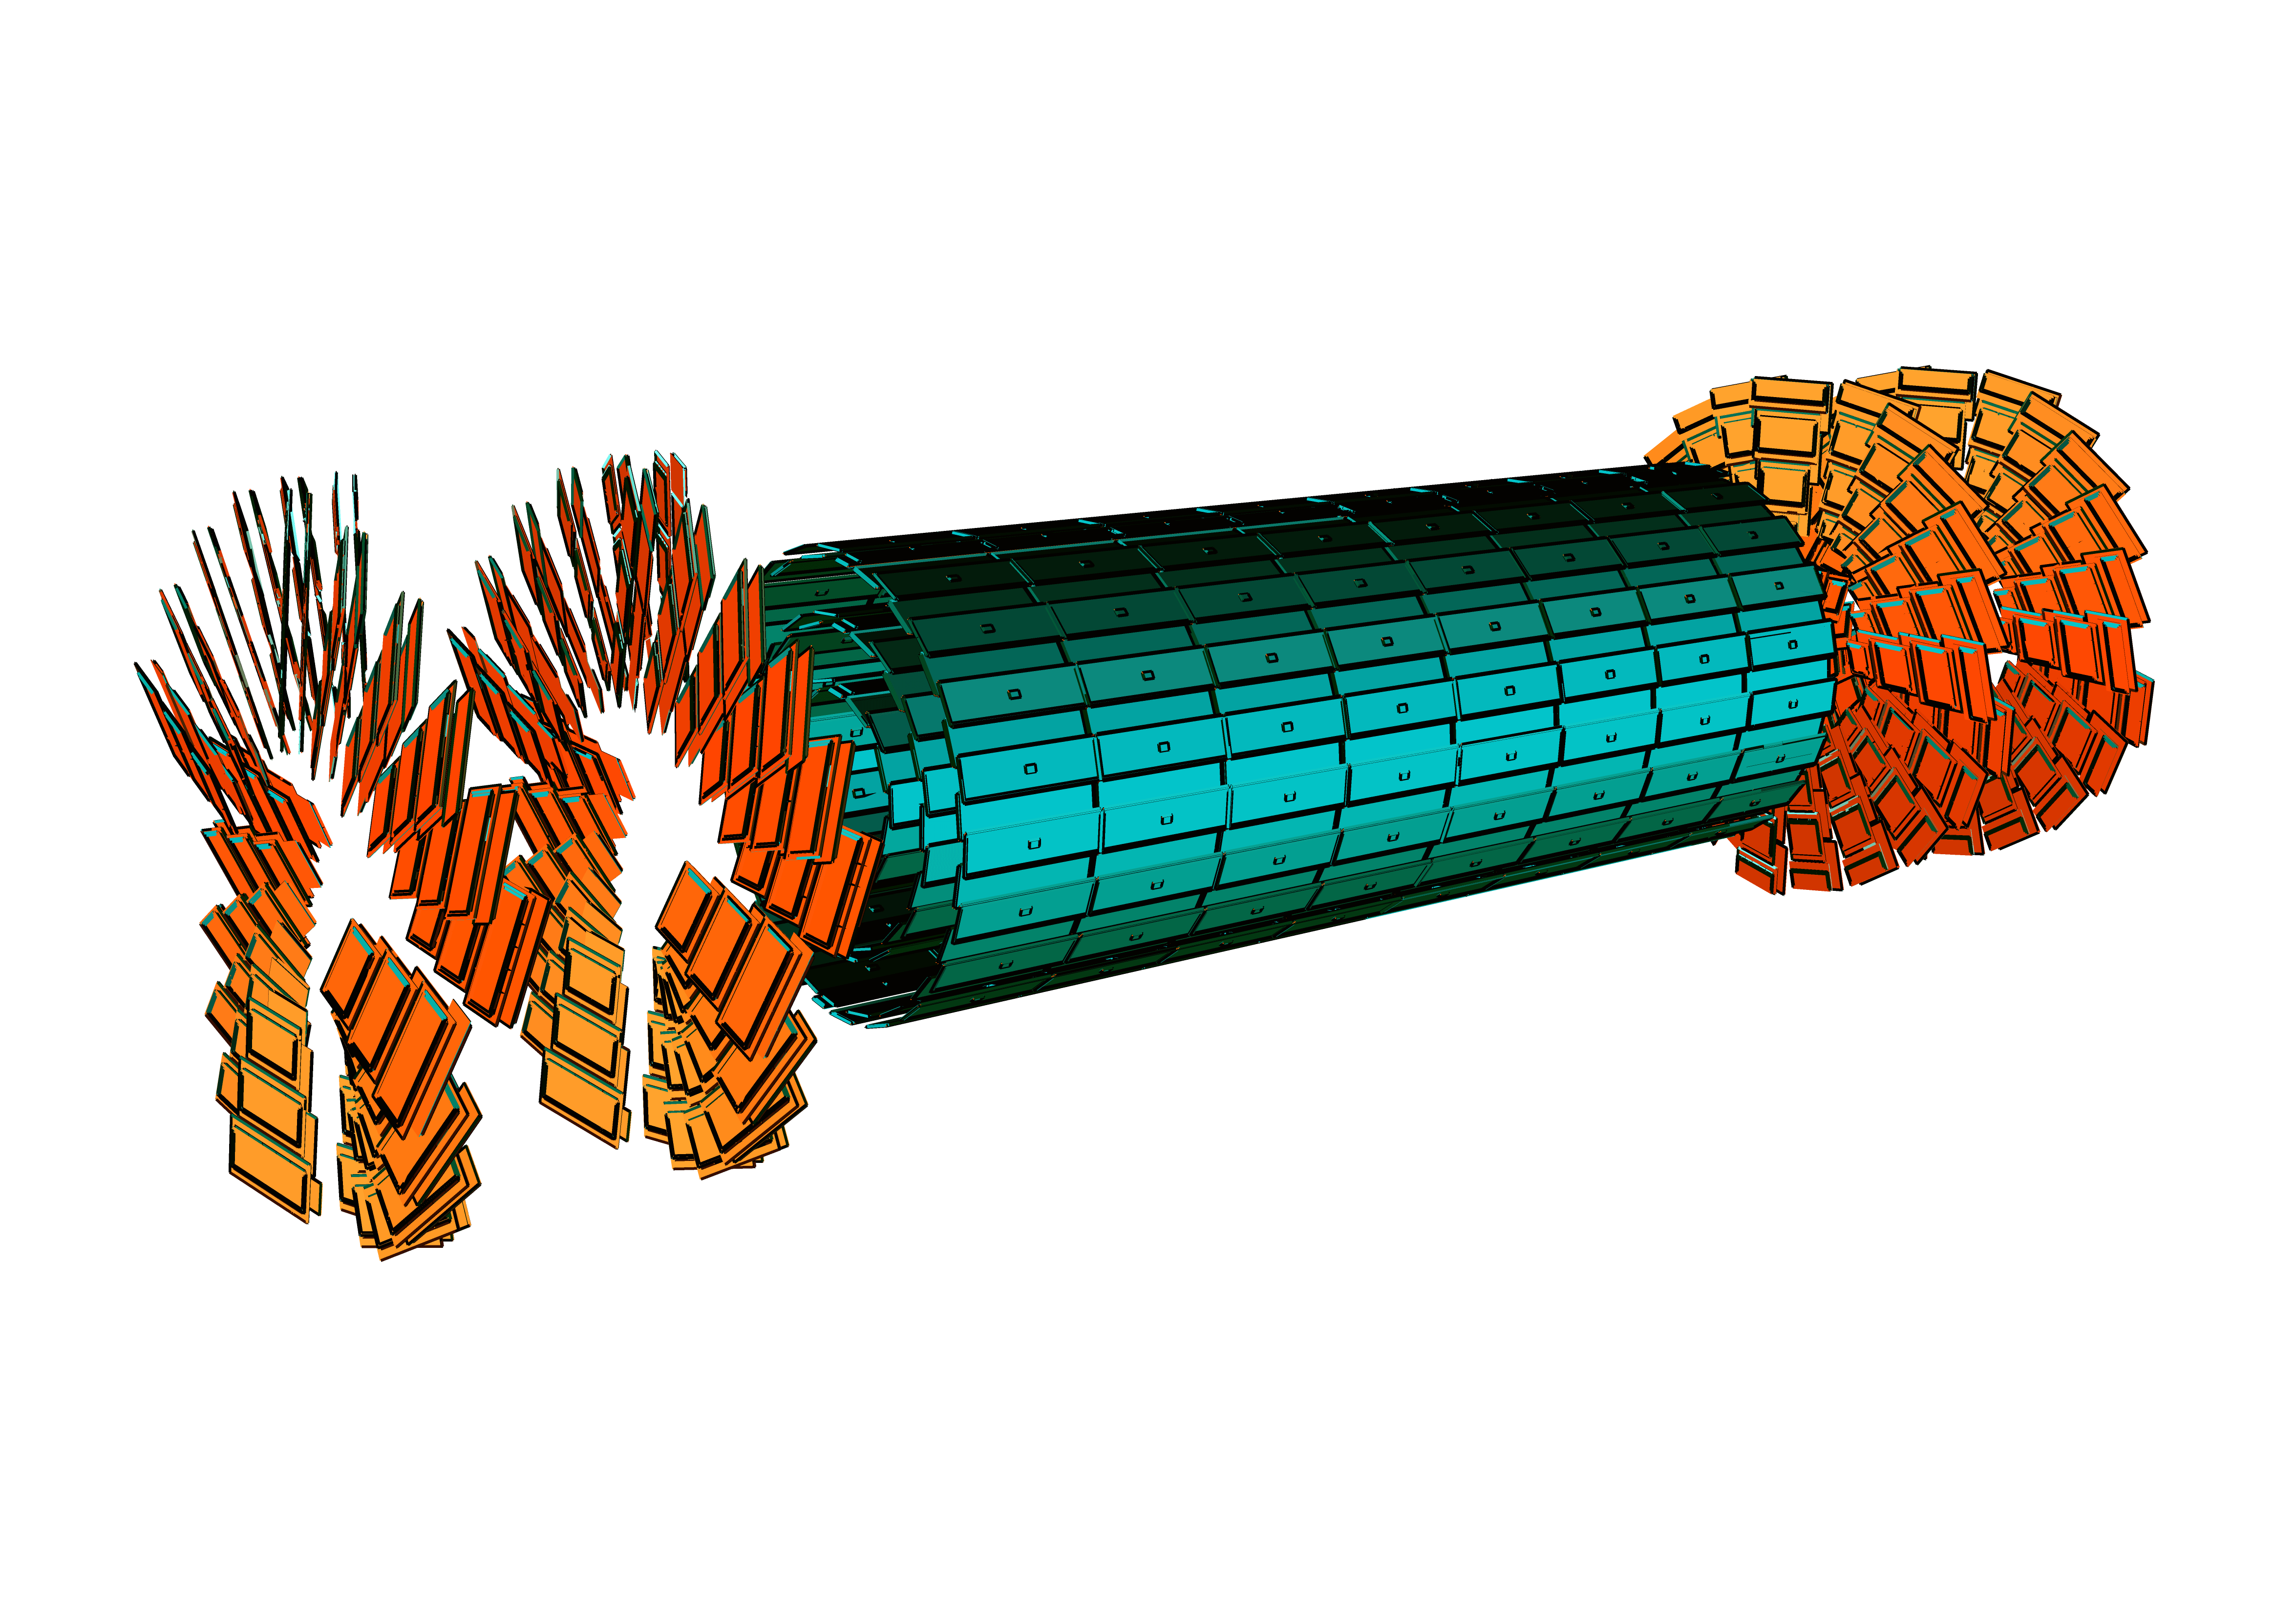
\includegraphics[width=0.8\textwidth]{Figures/pixel_detector.png}
		%\rule{35em}{0.5pt}
	\caption[CMS Pixel Detector]{A drawing of the CMS pixel detector. \cite{Chatrchyan:2008aa}}
	\label{fig:pixels}
\end{figure}
\begin{figure}[htbp]
	\centering
		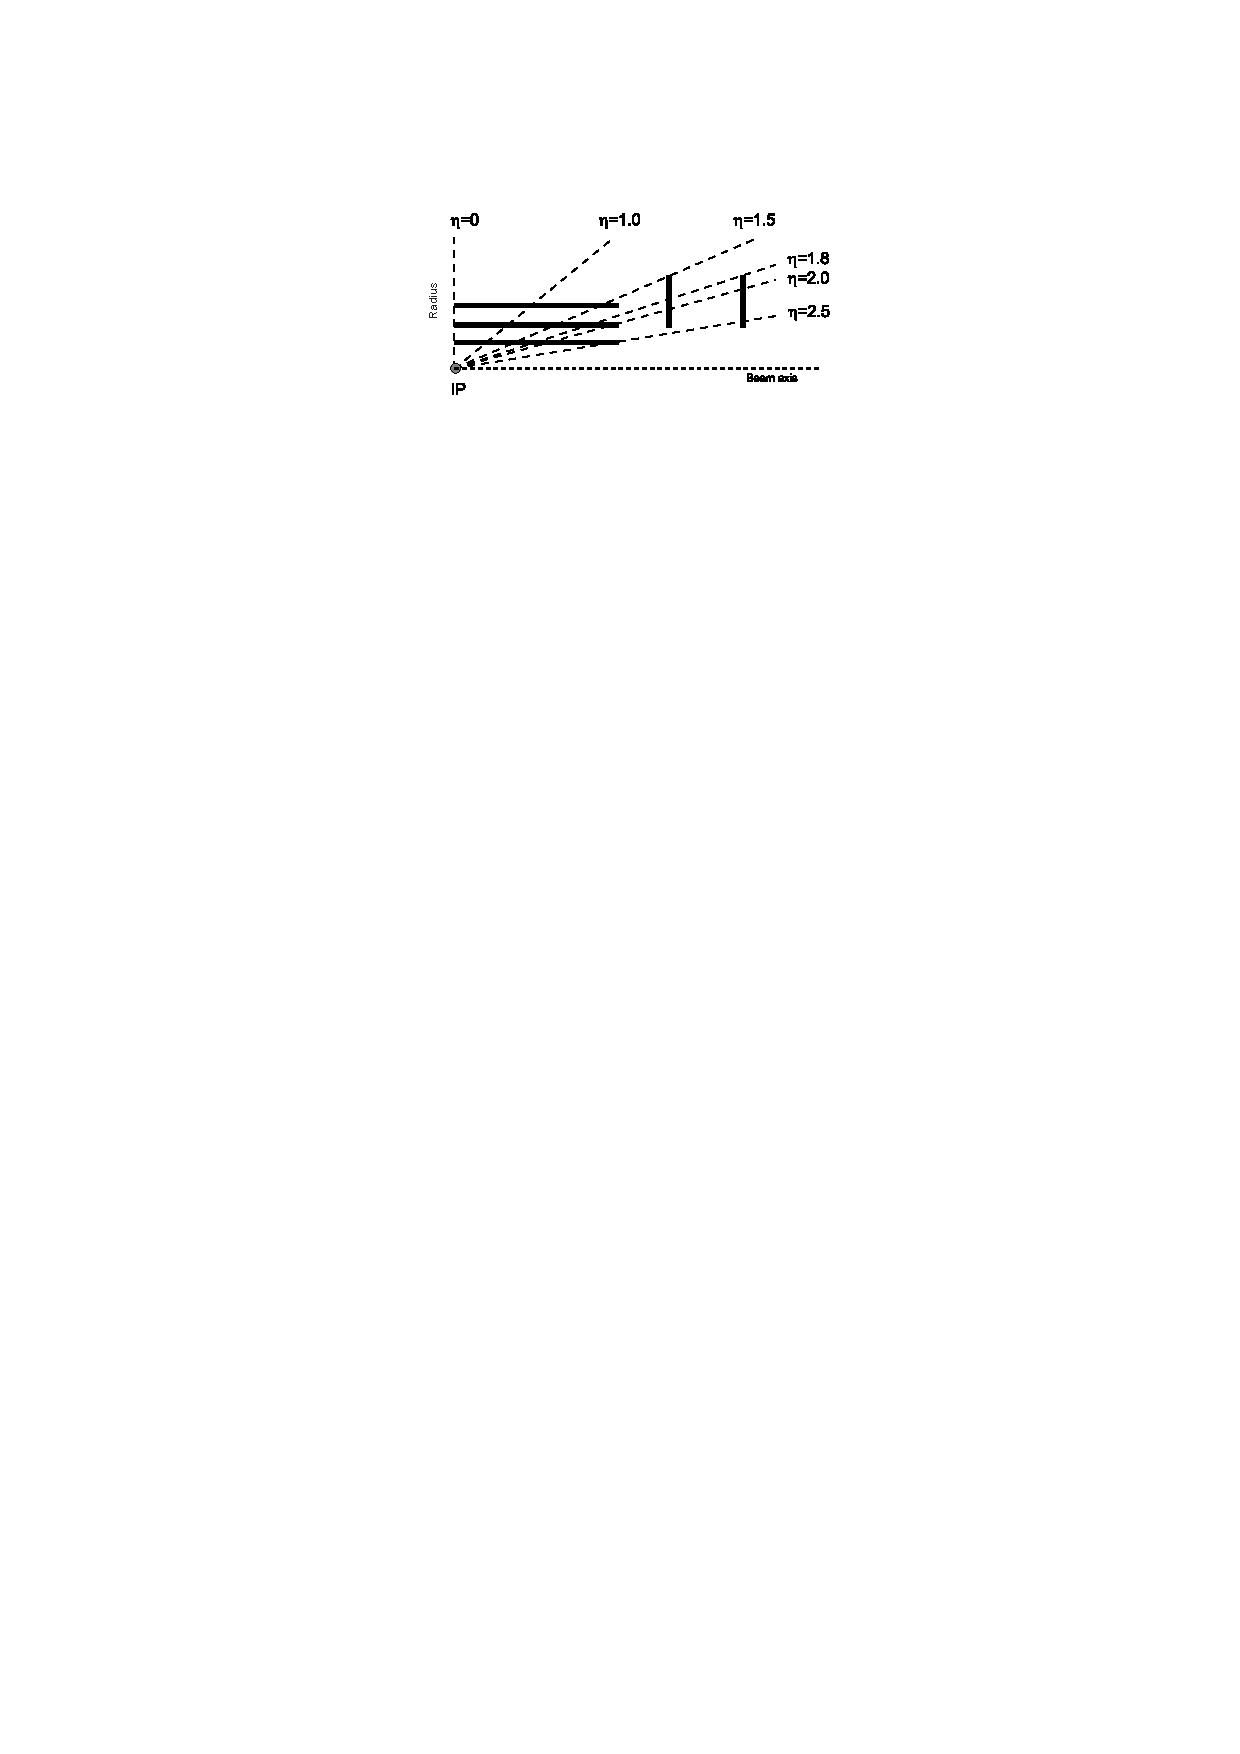
\includegraphics[width=0.49\textwidth]{Figures/pixel_eta.pdf}
		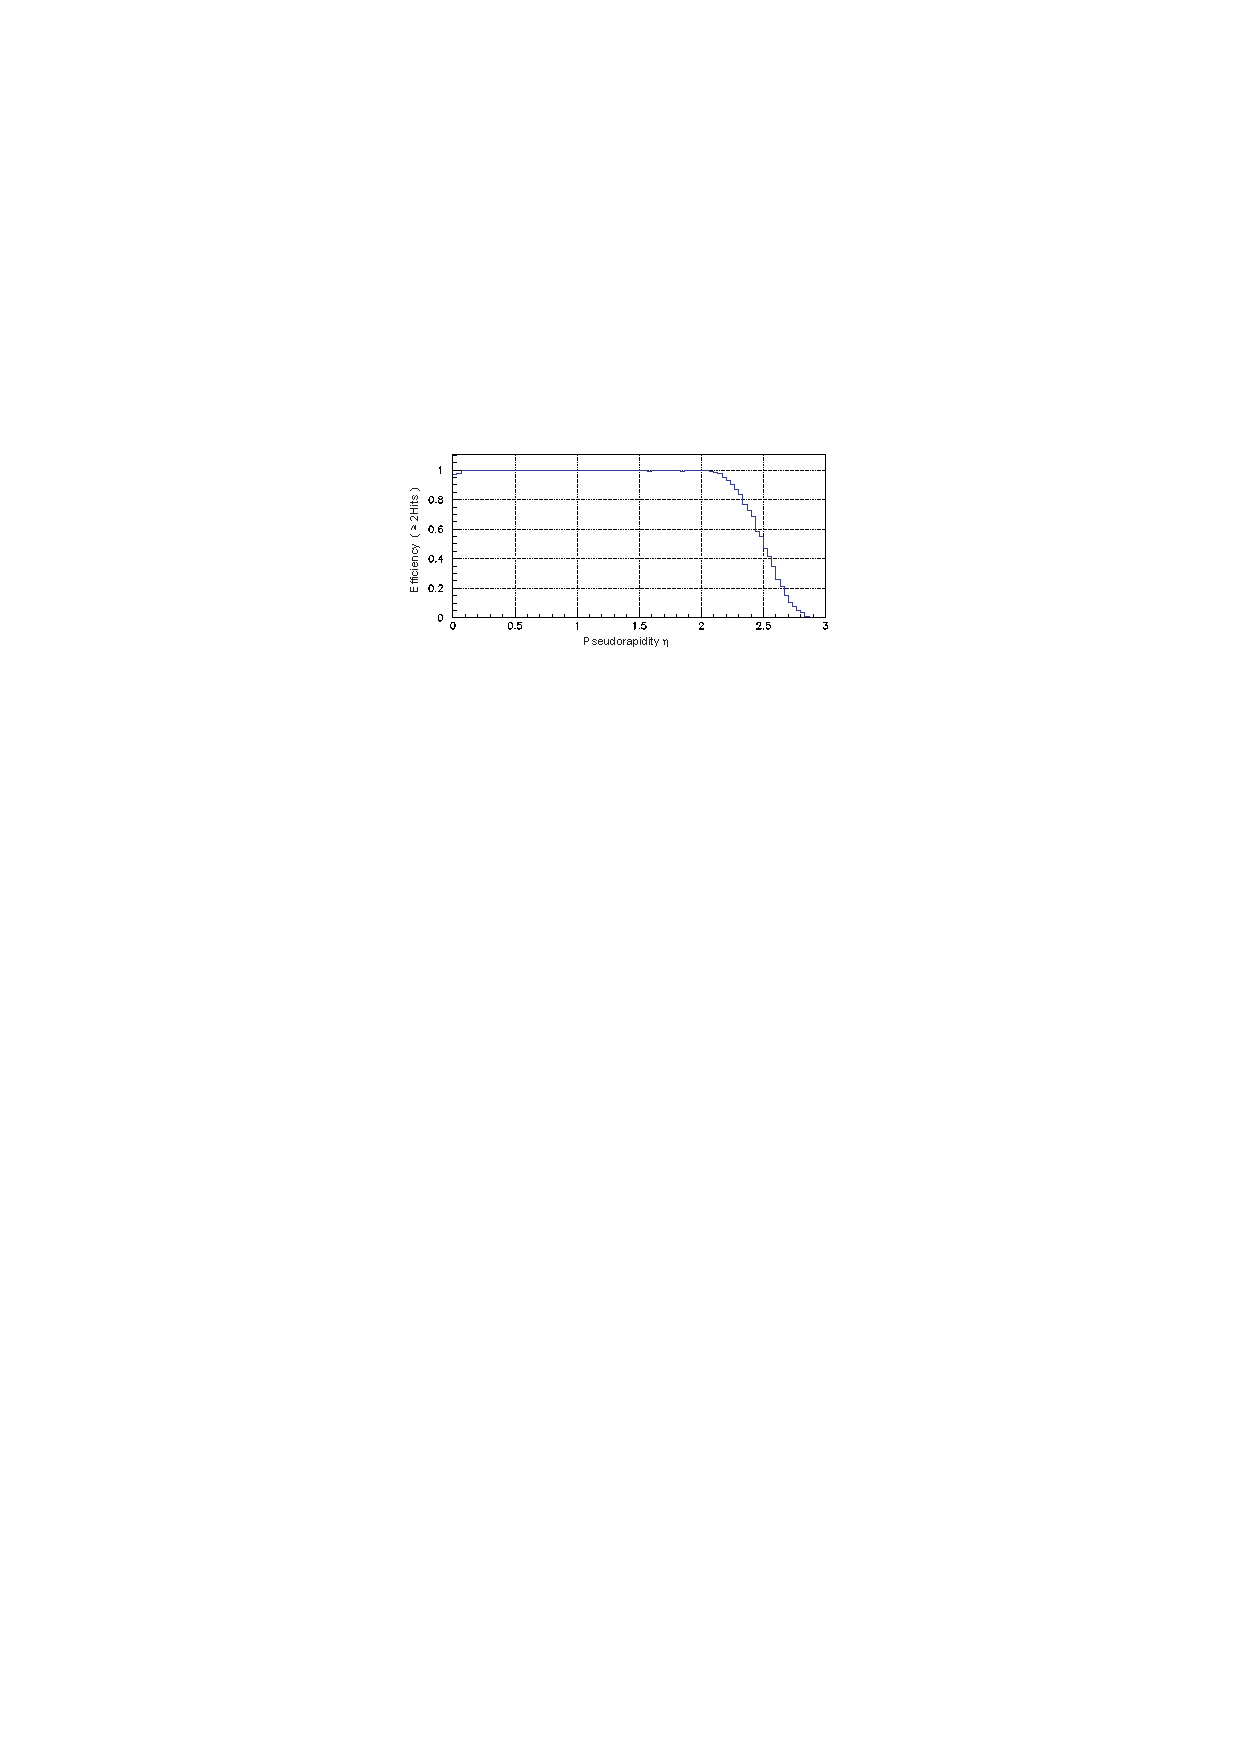
\includegraphics[width=0.49\textwidth]{Figures/pixel_eta2.pdf}
		%\rule{35em}{0.5pt}
	\caption[CMS Pixel Detector psudorapidity range coverage and efficiency]{A sketch of CMS Pixel Detector psudorapidity range coverage(\textit{left}) and hit efficiency as a function of pseudorapidity(\textit{right}). \cite{Chatrchyan:2008aa}}
	\label{fig:pixels_eta}
\end{figure}
\par Pixel detector is fully modular, consisting of rectangular modules in barrel part and quasi-triangular modules in the discs. Modules are arranged in a way to ensure measurements in at least three layers for each of the trajectories passing through the detector. Pixel size of $100\times150$ $\mu$m$^2$ results in similar resolution in $z$ and $r-\phi$ directions. In the barrel part the resolution of $15-20$ $\mu$m is achieved due to  charge sharing. Electrons inside the silicon shift under Lorentz force which is used in the reconstruction to determine the correct hit position. Detailed measurement of the Lorentz angle is described in the Appendix \ref{app:LA}. Pixel detector consists of 66 million pixels in total with 48 million being in the barrel pixel and 18 million in the forward. The closeness to the interaction point implies high track occupancy and necessity for radiation resistant materials. 
\par The readout of the pixel detector goes through read-out chips (ROC) to which each pixel is bump bonded and read out individually. There are around 16000 ROCs in the detector. Each ROC consists of 52$\times$80 pixels. Only pixels with signal above certain threshold are read out which can be tuned manually for each pixel. The average noise level in the detector is around 170 electrons at T$=-$10$^\circ$C. The information for each event is stored in a temporary buffer awaiting the signal from the Level-1 trigger in order to be read-out. Data is read out serially, with packets containing all hits corresponding to a single trigger. Each pixel hit uses six values, five to encode pixel position, and sixth value is the analog signal charge. ROC header is added at the beginning of each ROC sequence in order to make ROC hit-association possible. Signal is than digitized and sent to central data acquisition for further processing. Various other systems are installed in order to monitor and adjust the temperature, humidity, voltages, etc. 
\par With the design LHC luminosity, there are more than 1000 particles hitting the detector in every bunch-crossing. Very small pixel size results in the occupancy for each pixel of the order $10^{-4}$. The Pixel detector has been operational for several years and shows very little drop in performance due to irradiation. The plan is to keep the present detector during the Run 2, until 2017, and than replace it with new, four-layer pixel detector which is currently being built.

%-----------------------------------
%	SUBSECTION 2.2
%-----------------------------------

\subsection{Strip detector}

The silicon strip tracker is built in layers around Pixel detector where track particle flux is lower and a lower granularity detector can be used instead. The detector is built of strips in which a passing charged particle induces current. This resulting current is than transferred to silicon detectors connected to the wires. The barrel section of the strip detector consists of four layers in the inner part (TIB) and 6 layer in the outer part (TOB). In the forward regions there are three tracker inner discs (TID) on each side of the barrel and 9 layers in the tracker endcap (TEC). 
\par Some strips are built in double layers tilted against each other by an angle of 100 mrad to precisely measure the position of both $r\phi$ and $rz$ directions. The pitch size between strips varies from 80 $\mu m$ in the TIB to 184 $\mu$m in TOB and TEC. With the increasing distance from the interaction point, both strip pitch and strip length increase and sensor thickness becomes larger hence affecting the resolution.    

\begin{figure}[htbp]
	\centering
		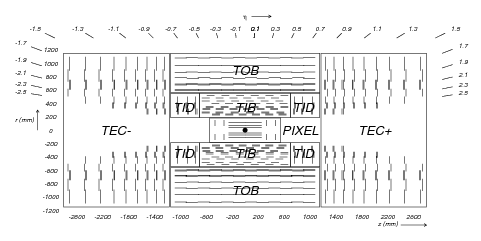
\includegraphics[width=0.9\textwidth]{Figures/strip_detector.png}
		%\rule{35em}{0.5pt}
	\caption[CMS Strip Detector]{A drawing of the CMS strip detector. \cite{Chatrchyan:2008aa}}
	\label{fig:strips}
\end{figure}

%----------------------------------------------------------------------------------------
%	SECTION 3
%----------------------------------------------------------------------------------------

\section{The electromagnetic calorimeter}

The electromagnetic calorimeter (ECAL) has the role of precisely measuring electrons and photons. It is built from lead tungstate (PbWO$_4$), a material with very high density (8.28 g$/$cm$^3$) and a small Moliere radius (0.89 cm) which is a scale characteristic of transverse dimension of the fully contained electromagnetic showers. The scintillation light emitted within a single bunch crossing of 25 ns is about 80$\%$ of the total light which means the response time of the detector is very small that represents a large advantage of this material. The calorimeters is built of 61 200 crystals in the barrel region and 14 670 crystals in the endcaps. Each crystal has a size of 22$\times $22 mm$^2$ in the front, 26$\times$26 mm$^2$ at the back side and length on 23 cm in the barrel region. In the endcaps, the size of the crystals varies from $28.62\times 28.62$ in the front to $30\times 30$ mm$^2$ in the back with a length of 22 cm. The whole systems covers the range $|\eta|<3$.
\begin{figure}[htbp]
	\centering
		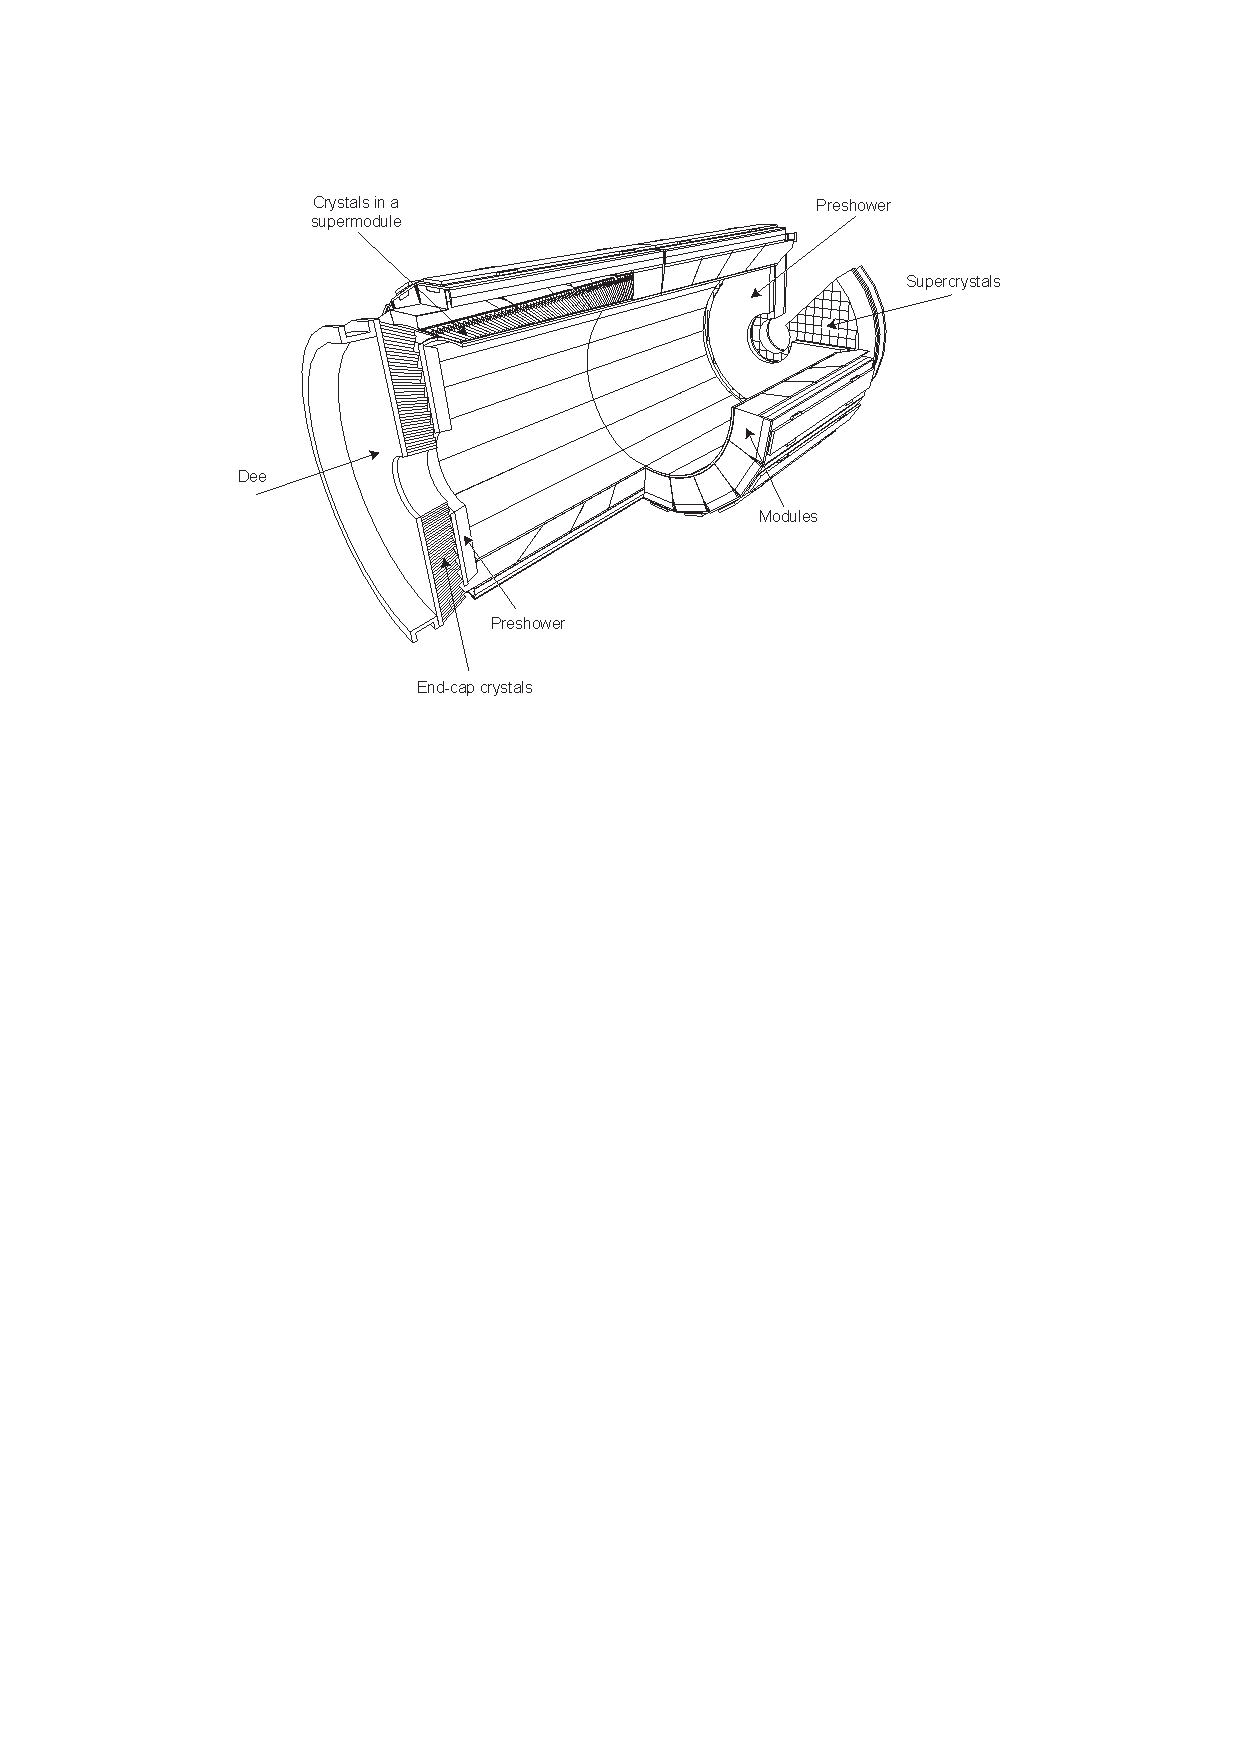
\includegraphics[width=0.8\textwidth]{Figures/ECAL.pdf}
		%\rule{35em}{0.5pt}
	\caption[CMS Electromagnetic Calorimeter]{A drawing of the CMS electromagnetic calorimeter. \cite{Chatrchyan:2008aa}}
	\label{fig:ECAL}
\end{figure}
\par Operation temperature of the detector is 18$^\circ$C at which $\sim$4.5 photoelectrons are collected per MeV of deposited energy. The blue-green scintillation light is measured by the avalanche photodiodes in the barrel and vacuum phototriodes in the endcaps.   
\par The ECAL energy resolution is affected by three uncorrelated sources and can be described by the relation \ref{eq:ECAL_res}. Parameters $a$, $b$ and $c$ are determined from the test beam. The stochastic term $a$ is very low for the lead tungstate crystals ($a$ = 2.83$\pm$0.3$\%$), which means that showers are mostly contained within the crystals. The noise term $b$ is determined from the electronics and amounts to $b=124$ MeV. The last term $c$ is the constant term which limits the ECAL accuracy at high energies.   
\begin{equation}
\left(\frac{\sigma_E}{E}\right)^2 = \left(\frac{a}{\sqrt{E}}\right)^2 + \left(\frac{b}{E}\right)^2 + c^2
\label{eq:ECAL_res}
\end{equation}   

%----------------------------------------------------------------------------------------
%	SECTION 4
%----------------------------------------------------------------------------------------

\section{The hadronic calorimeter}

The hadronic calorimeter (HCAL) is used to measure energies of hadron particles such as pions, kaons, protons, neutrons etc. Barrel and endcap hadronic calorimeters cover the pseudorapidity rande to $|\eta|=3$. 
Since the absorber in the transverse direction thickness is only 5.82 interaction lengths, additional layer was placed outside the solenoid and is called HO. HCAL is a sampling calorimeter which consists of layers of brass and plastic scintillator layers. Showers are produced mostly in brass and are detected in the scintillator and reemitted in the narrow wavelength range in which photodetectors operate. In the endcap region, steel and quartz are used because of their higher radiation hardness. There is an additional part of the detector placed 11.2 meters from the interaction point on both sides called forward HCAL which extends the coverage to $|\eta|=5.2$. Large HCAL coverage and good energy measurement are very important for jet reconstruction as well as for missing transverse energy determination.  
\begin{figure}[htbp]
	\centering
		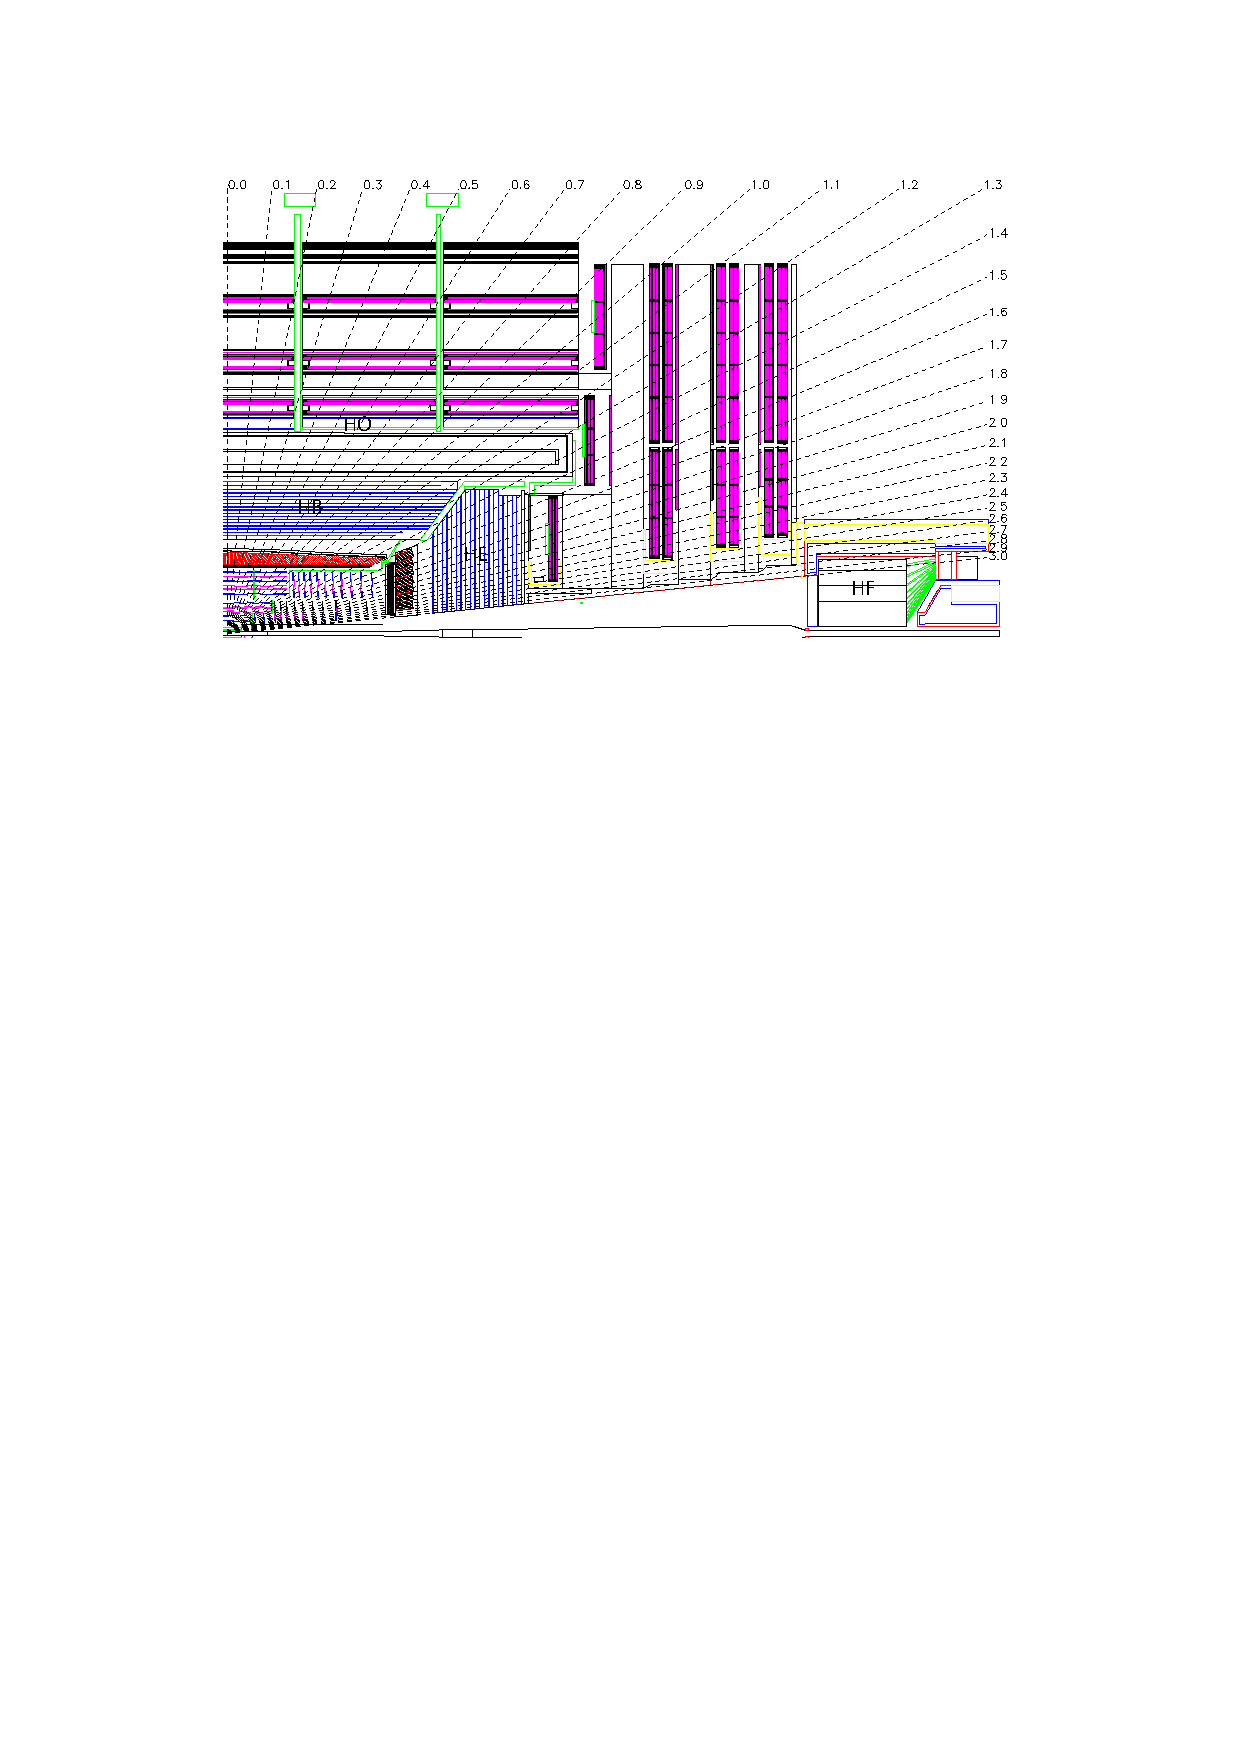
\includegraphics[width=0.8\textwidth]{Figures/HCAL.pdf}
		%\rule{35em}{0.5pt}
	\caption[CMS Hadronic Calorimeter]{A drawing of the CMS Hadronic Calorimeter. \cite{Chatrchyan:2008aa}}
	\label{fig:HCAL}
\end{figure}


%----------------------------------------------------------------------------------------
%	SECTION 5
%----------------------------------------------------------------------------------------

\section{The muon chambers}

Muons are the only particles that can pass the calorimeters and the solenoid. Their charge and momentum is measured also in the outer part of the detector by the muon chambers. There are three different types of the gaseous detectors used in the muon system, Drift tubes (DT), Resistive Plate Chambers (RPC) and Cathode Strip Chambers (CSC). Drift tubes are used in the barrel region where muon rate is relatively low and covers pseudorapidity range of $|\eta|<1.2$. The signal in Drift tubes is generated when a particle ionizes the gas inside the tube and the charge is collected by wires which are at high voltages. Cathode Strip Chambers are used in the endcap region where muon rate is much higher and magnetic field is not uniform. These are multi-wire proportional chambers with anodes that collect charge from the gas ionization. Resistive Plate Chambers are placed both in barrel and endcap region. These detectors are designed as two parallel plates which create a uniform electric field in the gas between them. The electrodes on the plates are highly resistive so  when charged particle passes, it causes an electron avalanche which passes through the plates and is collected by the external metallic strips. Their time resolution is of the order $\sim$1 ns which makes RPCs a good choice for triggering although their spatial resolution is not so good.
\begin{figure}[htbp]
	\centering
		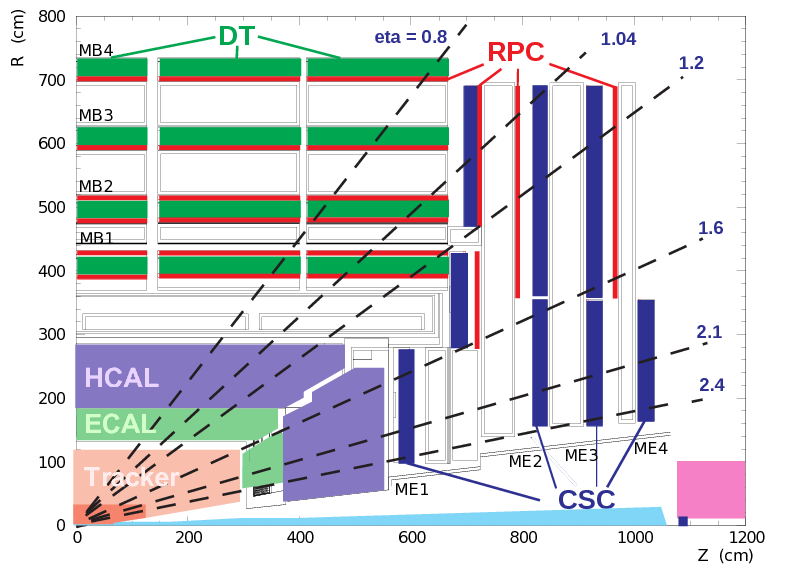
\includegraphics[width=0.8\textwidth]{Figures/Muon_chambres.png}
		%\rule{35em}{0.5pt}
	\caption[CMS Muon Chambers]{A drawing of the CMS muon chambers which consist of three different types of the detectors: Drift tubes, Cathode Strip Chambers and Resistive Plate chambers. \cite{Chatrchyan:2008aa}}
	\label{fig:Mu}
\end{figure} 
\par Large magnetic field enables even for high $p_T$ muons to be measured with a reasonable cell size in the muon chambers. The limiting factor for a good resolution of low $p_T$ muons is multiple scattering, and for high $p_T$ muons the chamber resolution. The momentum resolution as a function of muon $p_T$ is shown in Figure \ref{fig:MU_pt} for both muon chambers and inner tracking as well as the combined result. 
\begin{figure}[htbp]
	\centering
		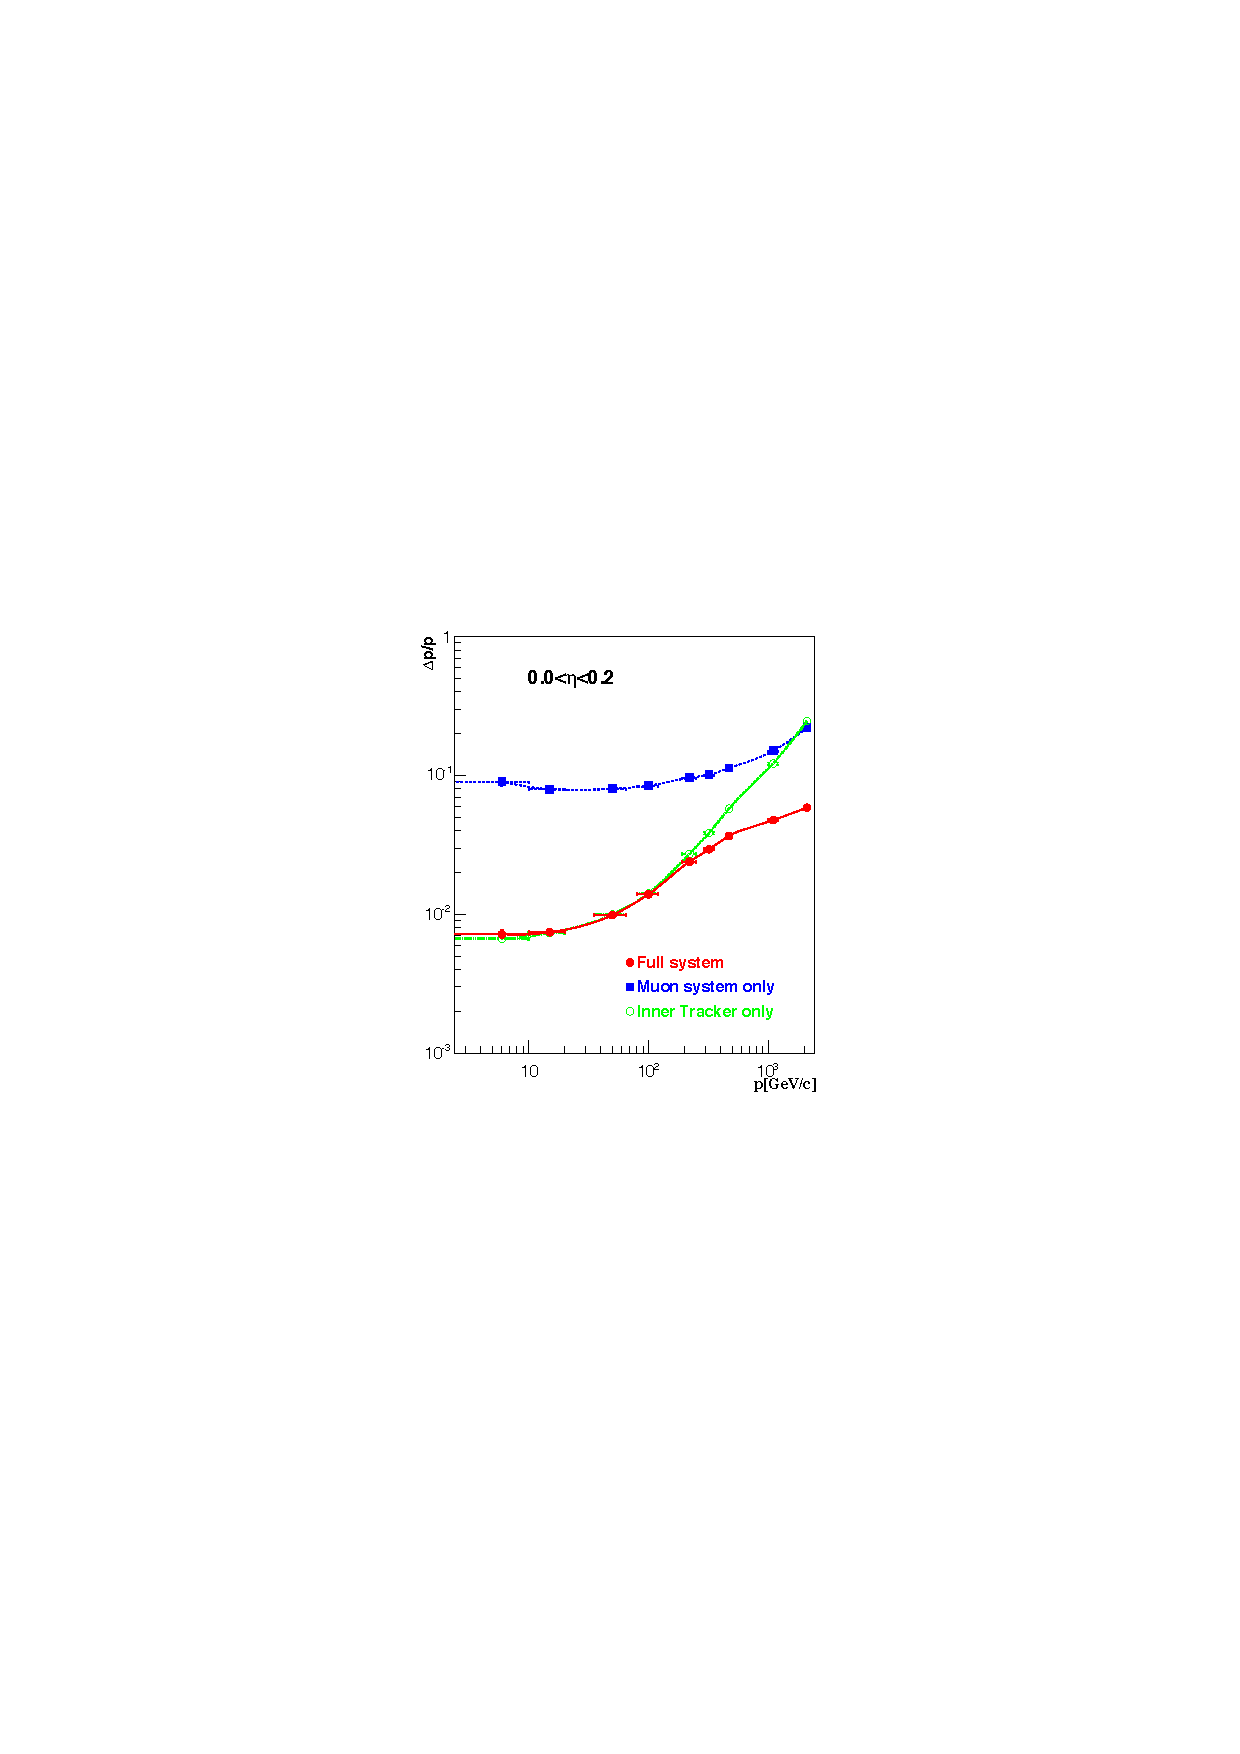
\includegraphics[width=0.5\textwidth]{Figures/MU_pt_res.pdf}
		%\rule{35em}{0.5pt}
	\caption[Muon resolution measurements for tracker, muon chambers and combined]{Muon resolution measurements for tracker, muon chambers and combined \cite{Chatrchyan:2008aa}}
	\label{fig:MU_pt}
\end{figure} 


%----------------------------------------------------------------------------------------
%	SECTION 6
%----------------------------------------------------------------------------------------

\section{The trigger}

The design rate of the proton collisions at the LHC is 40 MHz, although during Run 1 data taking period, the rate was 20 MHz which corresponds to 50 ns bunch spacing. Data collected in the same bunch crossing is called an event. Since there are huge amounts of data coming from the subdetectors, it is necessary to apply some selections which can reduce the rate to about 100 events per second. This is done by two level triggering system, the first one called Level 1 (L1) trigger and the second one called High Level Trigger (HLT). L1 trigger uses a special custom made electronics designed to reduce the output rate from 40 MHz to 100 kHz. Events which pass some loose criteria are than passed to the HLT. The L1 trigger uses the information from calorimeters and muon chambers to take the decision whether the event should be accepted or rejected usually searching for the presence of muons, jets above certain $p_T$, or looking at the total amount of $E_T$ and $E_T^{miss}$. The time needed to send the signals to the electronics, run the L1 selection and send the information back to the subdetectors in 3.2 $\mu$s. If the L1 trigger accepts the event, that is stored in the readout buffers where partial reconstruction takes place and the event is than processed by the HLT, which is a software farm that reduces the number of events to about 100 per second. The schematic of the trigger system is shown in figure \ref{fig:trigger}.
\begin{figure}[htbp]
	\centering
		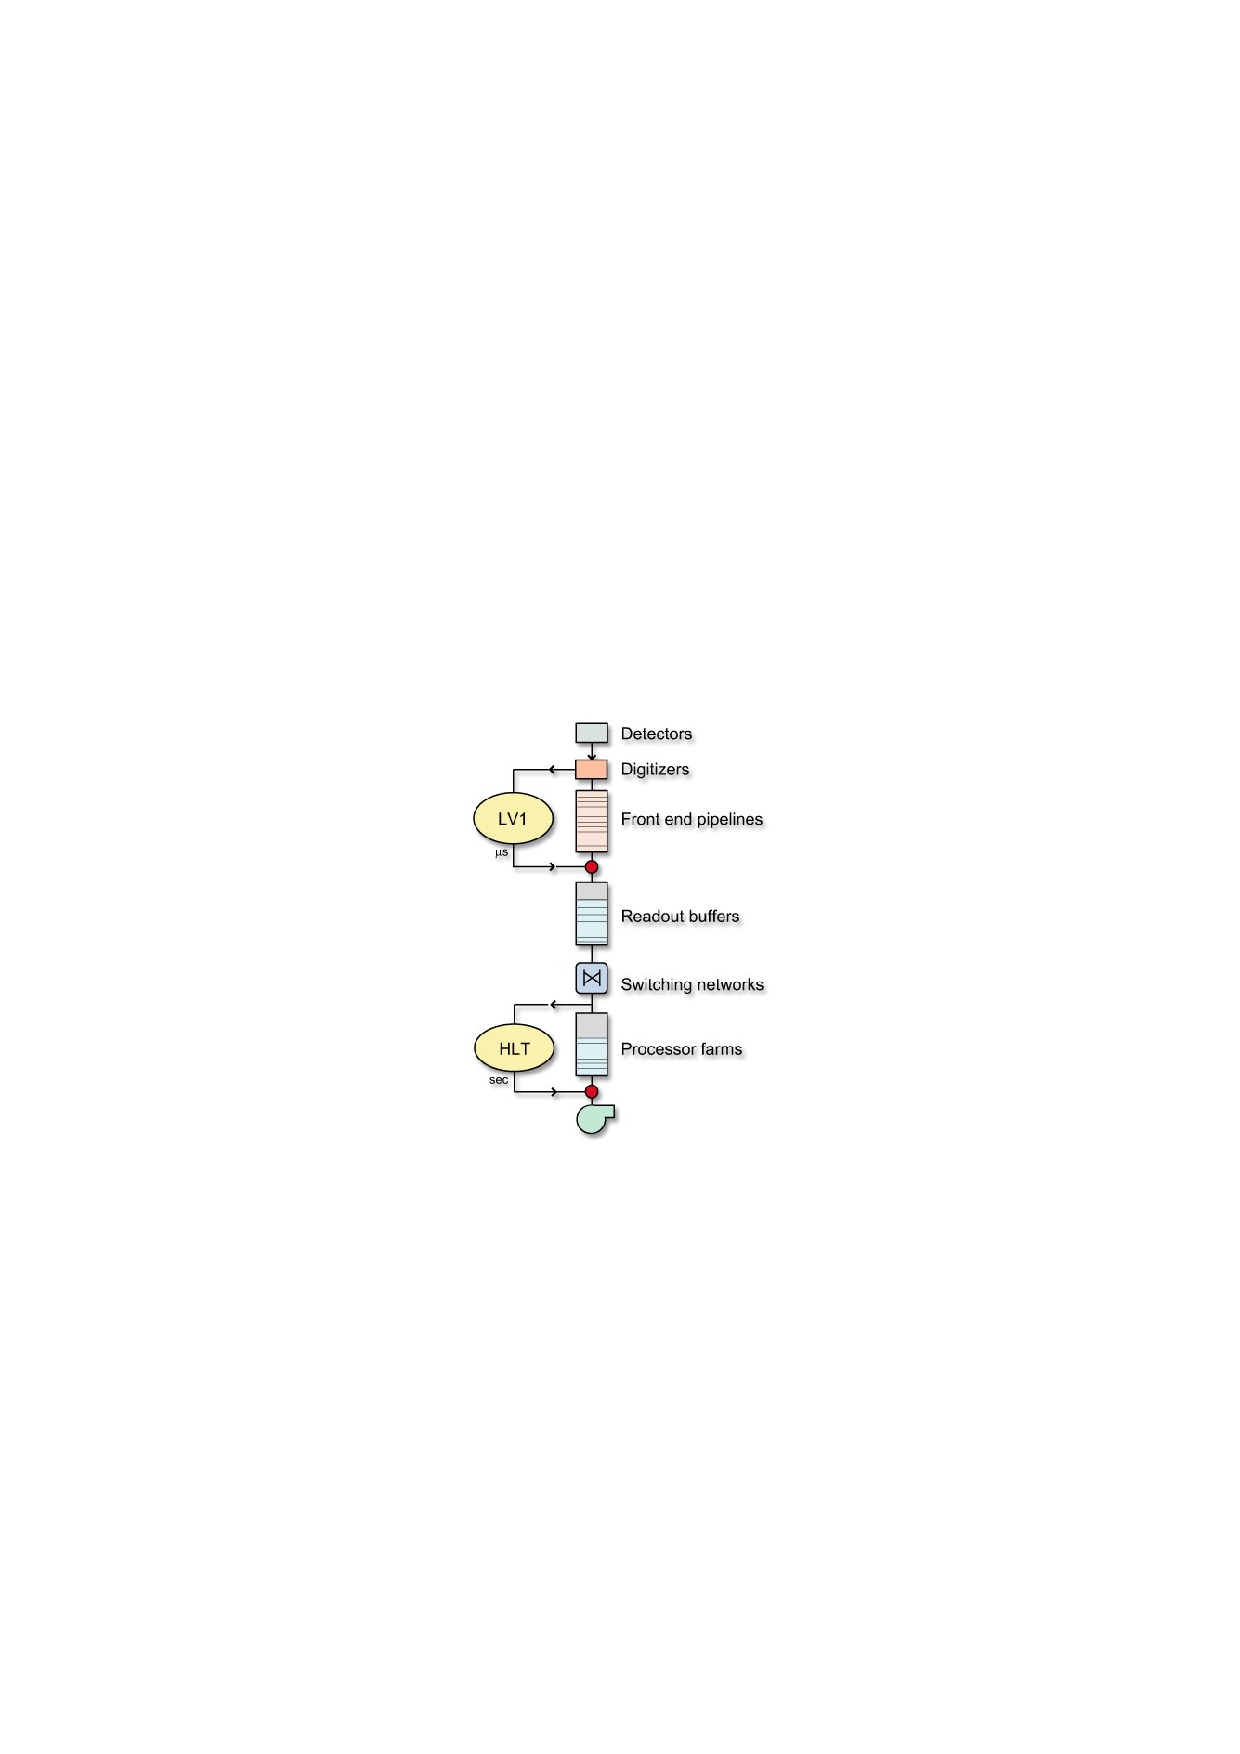
\includegraphics[width=0.4\textwidth]{Figures/trigger.pdf}
		%\rule{35em}{0.5pt}
	\caption[A drawing of CMS Trigger System.]{A schematic of CMS Trigger System. \cite{Chatrchyan:2008aa}}
	\label{fig:trigger}
\end{figure}

%----------------------------------------------------------------------------------------
%	SECTION 7
%----------------------------------------------------------------------------------------

\section{Luminosity measurement}
\label{sec:lumi}

Accurate and precise luminosity measurement is essential for physics analyses. CMS measurement is based either on the activity in the forward hadronic calorimeter (HF) or on the number of clusters in the pixel detector.
The forward calorimeter is placed in the high pseudorapidity region, covering range $3<|\eta|<5$. The measurement relies on the fraction of nonempty calorimeter towers to estimate the number of interactions. The uncertainty to this measurement comes from the nonlinear response of the HF to luminosity and the occurrence of the afterglow, the effect when the energy deposits created in a given bunch crossing produce a signal in subsequent bunch crossings. 
\par Luminosity measurement with the pixel detector is described in detail in \cite{CMS-PAS-SMP-12-008,CMS:2013gfa}. This method relies on the effective cross section measurement for pixel clusters determined with Van der Meer scan. This scan determines the shape and size of the interaction region by moving the beams across each other in transverse plane thus measuring the maximum available collision rate. The value of this cross section is then used to determine integrated luminosity for each lumi-section (23.3 seconds). This approach is not suitable for online luminosity measurements as pixel bias voltage is not turned on until the stable beams are declared and the data is not available if the central data acquisition system is busy. On the other hand, in the offline analysis this is not a problem as the data recorded without the pixel detector is discarded anyway.    
The total luminosity delivered in 2012 was around 24 fb$^{-1}$ while the luminosity recorded by the CMS was around 22 fb$^{-1}$. Ideally these two numbers would be the same, but due to the downtime of data acquisition or some of the subsystems, some of the delivered luminosity is not recorded.  
\chapter{Physics objects definitions} % Main chapter title

\label{Chapter5} % Change X to a consecutive number; for referencing this chapter elsewhere, use \ref{ChapterX}

\lhead{Chapter 5. \emph{Physics object definitions}} % Change X to a consecutive number; this is for the header on each page - perhaps a shortened title

CMS detector is designed to efficiently identify and reconstruct interesting physics objects. The reconstruction procedure which takes as input the signals from all subdetectors and combines them to get physics objects is called \textit{particle flow}. \cite{CMS:2009nxa} This algorithm classifies all the objects into one of the following categories: charged hadrons, neutral hadrons, photons, electrons and muons. These are built from reconstructed tracks, energy deposits in the calorimeters and signals in the muon chambers creating a global event description. Additionally, a set of cuts is imposed on both input signals and reconstructed object in order to minimize the misidentification, e.g wrongly identifying electron as a jet. 
\par Following sections show electron and muon reconstruction procedures and identification criteria. Additionally, jet reconstruction procedure is described together with necessary jet corrections and b-tagging algorithms. After the reconstruction of all other objects, missing transverse energy is computed.

%----------------------------------------------------------------------------------------
%	SECTION 1
%----------------------------------------------------------------------------------------

\section{Electrons}

Electrons in CMS are detected as a tracks in tracking system and an energy deposit in the electromagnetic calorimeter. Two different algorithms are used for electron reconstruction, \textit{tracker driven} seeding which is more suitable for low $p_T$ electrons and electrons inside jets and \textit{ECAL driven} seeding optimized for high $p_T$ isolated electrons. Both approaches take electromagnetic crystals with deposited energy and join them into \textit{clusters}. Electron passing through the detector bends due to magnetic field and interacts with the detector material emitting \textit{bremsstrahlung} photons. ECAL energy deposits from these photons are spread in $\phi$ direction in very narrow $\eta$ range and combined with the existing cluster forming a \textit{supercluster}. Trajectories are reconstructed using modeling of electron energy loss in detector material and fitted with a Gaussian Sum Filter(GSF)\cite{2005JPhG31N9A}.
\par Matching ECAL superclusters and reconstructed tracks is where the two approaches differ. Tracker driven seeding uses track from the tracking system and tries to match it with the supercluster in the ECAL while ECAL driven seeding starts from the superclusters.
Each electron candidate has to pass various quality cuts in order to maximize the probability of identifying the electron coming from the hard interaction, and reject electrons from jets or conversion. These selection cuts can be divided into three categories: identification, isolation and conversion cuts. Details on electron reconstruction and performance can be found in \cite{CMS:2010bta}.

%-----------------------------------
%	SUBSECTION 1.1
%-----------------------------------
\subsubsection*{Electron identification}
\label{sec:eleID}

Electron identification procedure first focuses on good matching between reconstructed track and supercluster, by imposing cuts on angular distance $\Delta \eta$ and $\Delta \phi$ between the two. These variables are computed as absolute $\eta$ and $\phi$ distance between the supercluster and electron track extrapolated to the ECAL surface. Additionally, a cut is imposed on $\sigma_{i\eta i\eta}$ which describes a shower shape spread in $\eta$ direction. This variable is particularly discriminating against clusters coming from electrons and energy deposits from photons and fakes. Shower shape is defined as:
\begin{equation}
\sigma_{i\eta i\eta} = \sqrt{\frac{\sum_{i}^{5\times 5} w_i(\eta_i-\eta_{seed})^2\times \Delta \eta^2_{xtal} }{\sum_{i}^{5\times 5}}}
\end{equation}
where $i$ runs over all crystals in $5\times5$ block around supercluster seed, $\eta_i-\eta_{seed}$ is the distance in number of crystals in $\eta$ direction between $i$-th crystal in supercluster and seed crystal and $\Delta \eta^2_{xtal}$ is the average width of a single crystal. Each crystal is given a weight defined as $w_i=max(0,4.7+ln(E_i/E_{5\times5}))$, where $E_i$ is a single crystal energy, and $E_{5\times 5}$ is the sum of energy deposits inside a 5$\times$5 crystal block. 
Additional cut on the ratio between the energy deposits in the hadronic and electromagnetic calorimeter for electrons is used to discard the events with significant hadron activity.
\par Electrons coming from photon conversions are rejected by requiring a hit in every layer of the inner tracking system. Additionally, for each electron track a fit is performed trying to combine it with another electron track under the hypothesis that both electrons originate from converted photon. Electron is selected only if this probability is sufficiently small. Electron compatibility with the primary vertex is estimated by looking at the impact parameters in both $xy$ and $z$ planes. Due to the gap in the electromagnetic calorimeter in 1.4442 $< |\eta| <$ 1.566, all electrons which have a supercluster position reconstructed in this range are rejected. A full list of identification criteria is summarized in Table \ref{tab:eleID}.
 \begin{table}[h]
\centering
  \caption{A summary of electron identification criteria.}
  \label{tab:eleID}
  \begin{tabular}{ l  c c}
      \hline
      \hline
      	Variable & Barrel & Endcap \\
      	\hline
    		$\Delta\eta$ $<$ &  0.004 & 0.005 \\
     	$\Delta\phi$ $<$ &  0.03 & 0.02 \\
     	$\sigma_{i\eta i\eta}$ $<$ & 0.01 & 0.03 \\
		$H/E$ $<$ & 0.12 & 0.10 \\
		$d_{xy}$ $<$ & 0.02 cm & 0.02 cm \\
		$d_{z}$ $<$  & 0.1 cm & 0.1 cm \\
		$(1/E - 1/p)$ $<$ & 0.05 & 0.05\\
		Missing hits  & 0 & 1 \\
		Vertex Fit Probability & $10^{-6}$ & $10^{-6}$ \\    	

      \hline
      \hline 
  \end{tabular}
\end{table}


%----------------------------------------------------------------------------------------
%	SECTION 2
%----------------------------------------------------------------------------------------

\section{Muons}

Muons in CMS are reconstructed by combining a reconstructed track inside the tracker(\textit{tracker track}) and track in muon chambers (\textit{standalone muon track}). Individual track segments in the muon chambers are fitted using Kalman fitter technique \cite{Fruhwirth1987444}  in order to obtain a standalone muon track. Similar as with electrons, two approaches are used for combining track from tracker and standalone track. 
\par \textit{Global muon reconstruction} approach uses a standalone muon track in the muon chambers and tries to find a matching tracker track by combining parameters of two tracks by projecting it to the common surface. This \textit{outside-in} approach uses Kalman fitter technique to combine these two objects in an object called \textit{global muon}. Muon momentum is then determined from this global muon track using all available systems which shows improved precision in comparison to other approaches.  
\par The second approach for muon reconstruction is \textit{tracker muon reconstruction} which starts from tracks inside the tracker with $p_T>0.5$ GeV/c and total momentum $p>2.5$ GeV/c as potential muon candidates. Extrapolation is than performed to the muon chambers taking into account the magnetic field, Coulomb scattering in the material and other energy losses. \textit{Tracker moun} is found if at least one muon segment matches the extrapolated track. The efficiency of the \textit{Tracker muon} reconstruction is higher for low energy muons than the efficiency for the global muons, because only a single muon segment in the muon chambers is required. For high energy muons where more there are more segments inside muon chambers, \textit{global muon} algorithm is designed to have high efficiency. Detailed muon reconstruction procedure is shown in \cite{2012JInst7P0002T}.    

%-----------------------------------
%	SUBSECTION 2.1
%-----------------------------------

\subsubsection*{Muon identification}
\label{sec:muID}

In this analysis \textit{particle flow} muon identification selection is applied to the \textit{global muons}. Selection is applied in order to minimize misidentification of charged hadrons as muons, maximize the efficiency of muon identification inside jets and ensure good momentum measurement. Muons used in the analysis have $|\eta|<2.1$ and transverse momentum $p_T>30$ GeV with more than 5 hits in the inner tracker system and at least one hit in pixel detector. At least one good muon chamber hit in the \textit{global muon} track fit is required to have $\chi^2/ndof<10$, at least two segments in two different muon stations should be matched to a track in order to suppress muons from in-flight decays. Cosmic muons are rejected by applying cuts on the impact parameter with respect to the primary vertex of $|d_{xy}|<$0.2 cm and $|d_z|<$ 0.5 cm. Muon identification criteria are summarized in Table \ref{tab:muID}.

  \begin{table}[h]
\centering
  \caption{A summary of muon identification criteria.}
  \label{tab:muID}
  \begin{tabular}{ l  c c}
      \hline
      \hline
      	Variable & Requirement \\
      	\hline
    		number of pixel hits $>$ &  0 \\
     	number of inner tracker hits $>$ &  5 \\
     	$\chi^2/ndof$ $<$ & 10 \\
		number of muon hits $>$ & 0  \\
		chambers with matched segments $>$ & 1  \\		
		$d_{xy}$ $<$ & 0.2 cm \\
		$d_{z}$ $<$  & 0.5 cm \\
      \hline
      \hline 
  \end{tabular}
\end{table}
 

%-----------------------------------
%	SUBSECTION 2.2
%-----------------------------------

\section{Lepton isolation}
Leptons from W decays are in general expected to be well isolated. The degree of isolation is calculated using \textit{particle flow} approach by summing the transverse momenta contributions of particles around the lepton inside a specific cone. All charged particles are considered as well as photons and neutral hadrons with $p_T>$0.5 GeV. The cone used for determination of energy deposits is defined as $\Delta R = \sqrt{\Delta \phi^2+ \Delta \eta^2}$ around the lepton axis and isolation measure is defined as:
\begin{equation}
I_{PF}^{rel} = \frac{\sum p_T^{charged} + max(0, \sum E_T^{\gamma}+\sum E_T^{neutral}-0.5\sum E_T^{PU})}{p_T^l}
\end{equation}
where $p_T^{charged}$ is the sum of the momenta of charged hadrons and $E_T^{\gamma} $ and $E_T^{neutral}$ are the sums of photon and neutral hadron momenta. $E_T^{PU}$ is the sum of the pile-up transverse energies from neutral particles and is calculated as a sum of track transverse momenta not coming from the primary vertex inside the isolation cone. This is divided by the factor of 0.5 which corresponds approximately to the ratio of neutral to charged hadron production in the hadronization process of pile-up interactions. Selected muons are required to pass isolation cut $I_{rel}^{PF}<0.12$. On the other hand, if there is a requirement that there be no leptons in the event, the isolation cut is $I_{PF}^{rel}<0.2$. Electron isolation is computed in the same way with cut of $I_{rel}^{PF}<0.1$ for selected electrons and $I_{rel}^{PF}<0.15$ for vetoed additional electrons.


%----------------------------------------------------------------------------------------
%	SECTION 3
%----------------------------------------------------------------------------------------

\section{Jets}

In high energy physics, jet is a collimated group of hadrons which emerges as a result of quark or gluon fragmentation and hadronization process. Hadrons reconstructed in a particle detector need to be combined in order to form a jet and give information about the initial parton. A set of rules has to be created which define how to group particles and how to assign momentum to the jet. Usually this is done by summing the four-momentum of each particle in a jet.

%-----------------------------------
%	SUBSECTION 3.1
%-----------------------------------

\subsection{Jet algorithms}

Jet algorithms take into account the distance between particles and define rules to determine which particle belongs to what jet. Same jet algorithms should be applicable to both, experimental data and theoretical calculation.  Other important properties of jet algorithms are \textit{infrared safety} and \textit{collinear safety} which means if an event is modified by addition of soft emission of collinear splitting, the final number of hard jets will remain unchanged. These two properties together are called \textit{IRC safety}. IRC unsafe jet algorithms may break the cancellation of divergences by yielding one set of jets for tree-level splitting while loop diagrams lead to another, as shown if figure \ref{fig:jet_unsafe}, giving infinite cross-sections in the final calculations. Jet definitions, jet relation to partons and an overview of different jet algorithms are summarized in \cite{Salam:2009jx}.
\begin{figure}[htbp]
	\centering
		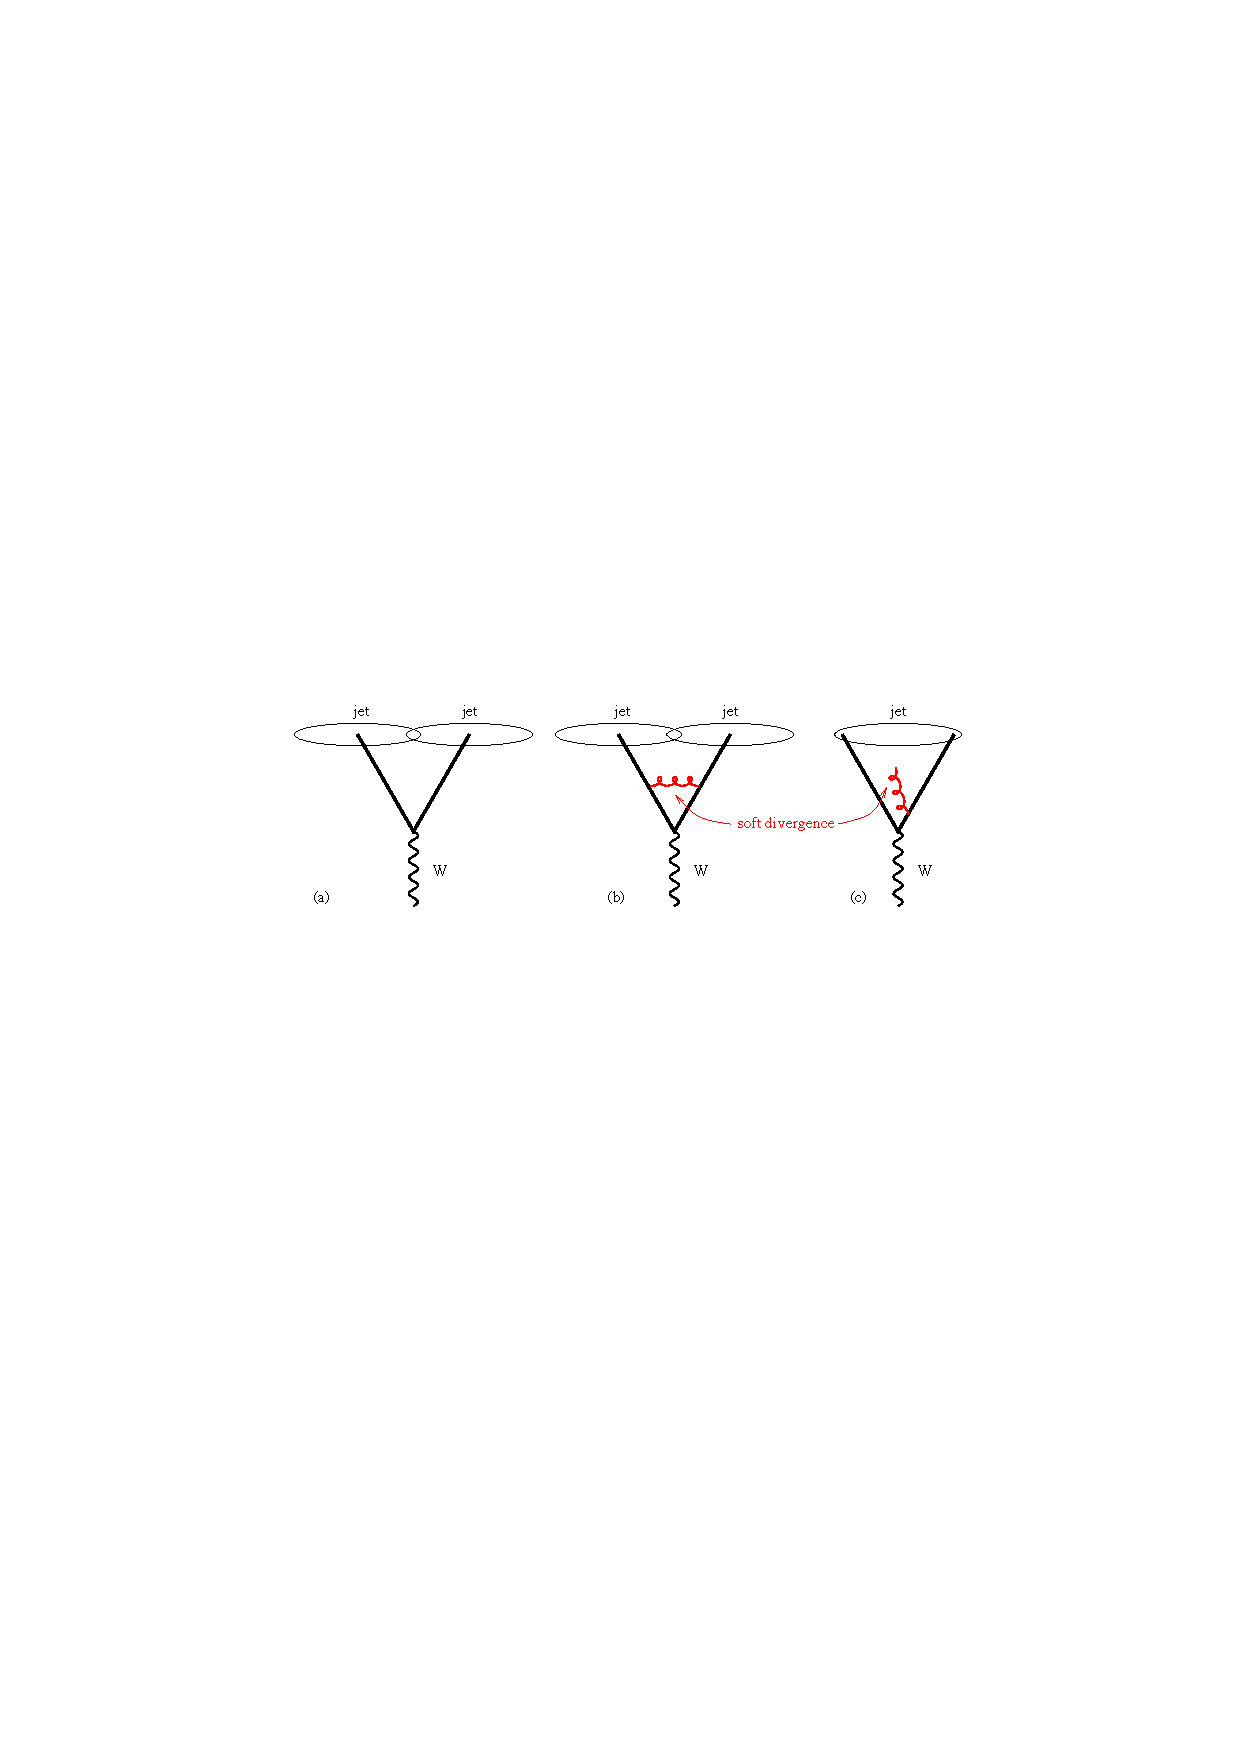
\includegraphics[width=0.8\textwidth]{Figures/jet_unsafe2.pdf}
		%\rule{35em}{0.5pt}
	\caption[An example of configuration of IRC unsafe jet algorithm.]{Configuration showing IC  unsafety with W boson and two partons. Adding a soft gluon causes two jets to be reconstructed as one. \cite{Salam:2009jx}}
	\label{fig:jet_unsafe}
\end{figure}

\par There are two types of jet algorithms which are most commonly used: \textit{cone algorithms} and \textit{sequential recombination algorithms}. In the case of \textit{cone algorithms}, a jet is defined as a set of particles inside a stable cone around their center of mass. Most popular cone algorithm is \textit{iterative cones} (IC) where a seed particle is chosen and momenta of all particles around that initial particle inside a cone of radius $R$ are summed. After adding each new particle to the sum, the direction of the new sum is taken as a seed direction, and the procedure repeats until the direction of the resulting cone is stable. Particles inside the cone are than removed from the list of available particles and the procedure repeats. This approach is not IRC safe given that nearly collinear splitting of the hardest particle in the event can be reconstructed as two jets. In that case, a less energetic, particle, pointing in another direction, can become the hardest particle in the event, yielding different set of jets. Cone algorithms can be IRC safe using a \textit{seedless cone} (SC) algorithm where all stable cone solutions are identified at once. However this approach is very time consuming even for small number of particles and thus very impractical to use.
In the \textit{sequential recombination algorithms} at hadron colliders two longitudinally invariant distances are introduced: $d_{ij}$ which is the distance between each pair of particles and $d_{iB}$ which is the particle-beam distance. These distances are defined as: 
\begin{equation}
d_{ij} = min(k_{T,i}^{2p},k_{T,j}^{2p}) \frac{\Delta R_{ij}^2}{R^2}
\end{equation}
\begin{equation}
d_{iB}=k_{T,i}^{2p}
\end{equation}
where $\Delta R_{ij}$ denotes the distance in the $\eta -\phi$ plane and is computed as $$\Delta R_{ij}^2 = (\eta_i-\eta_j)^2+(\phi_i-\phi_j)^2.$$ $k_T$ is transverse momentum of the particle, $R$ is an angular cut-off similar to the one in \textit{cone algorithms},  and $p$ defines which particles are clustered first and is described below. Both $R$ and $p$ are free parameters of the algorithm. The algorithm is applied using the following approach: first two distances $d_{ij}$ and $d_iB$ are computed and minimal values are found. If $d_{ij}$ is smaller, that two particles are combined, treated as a new particle and the distance with next particle in the list is computed. In case of $d_iB$ being smaller, $i$ is declared to be the final jet is removed from the list of particles. The procedure continues until there are no more particles in the list.
\begin{figure}[htbp]
	\centering
		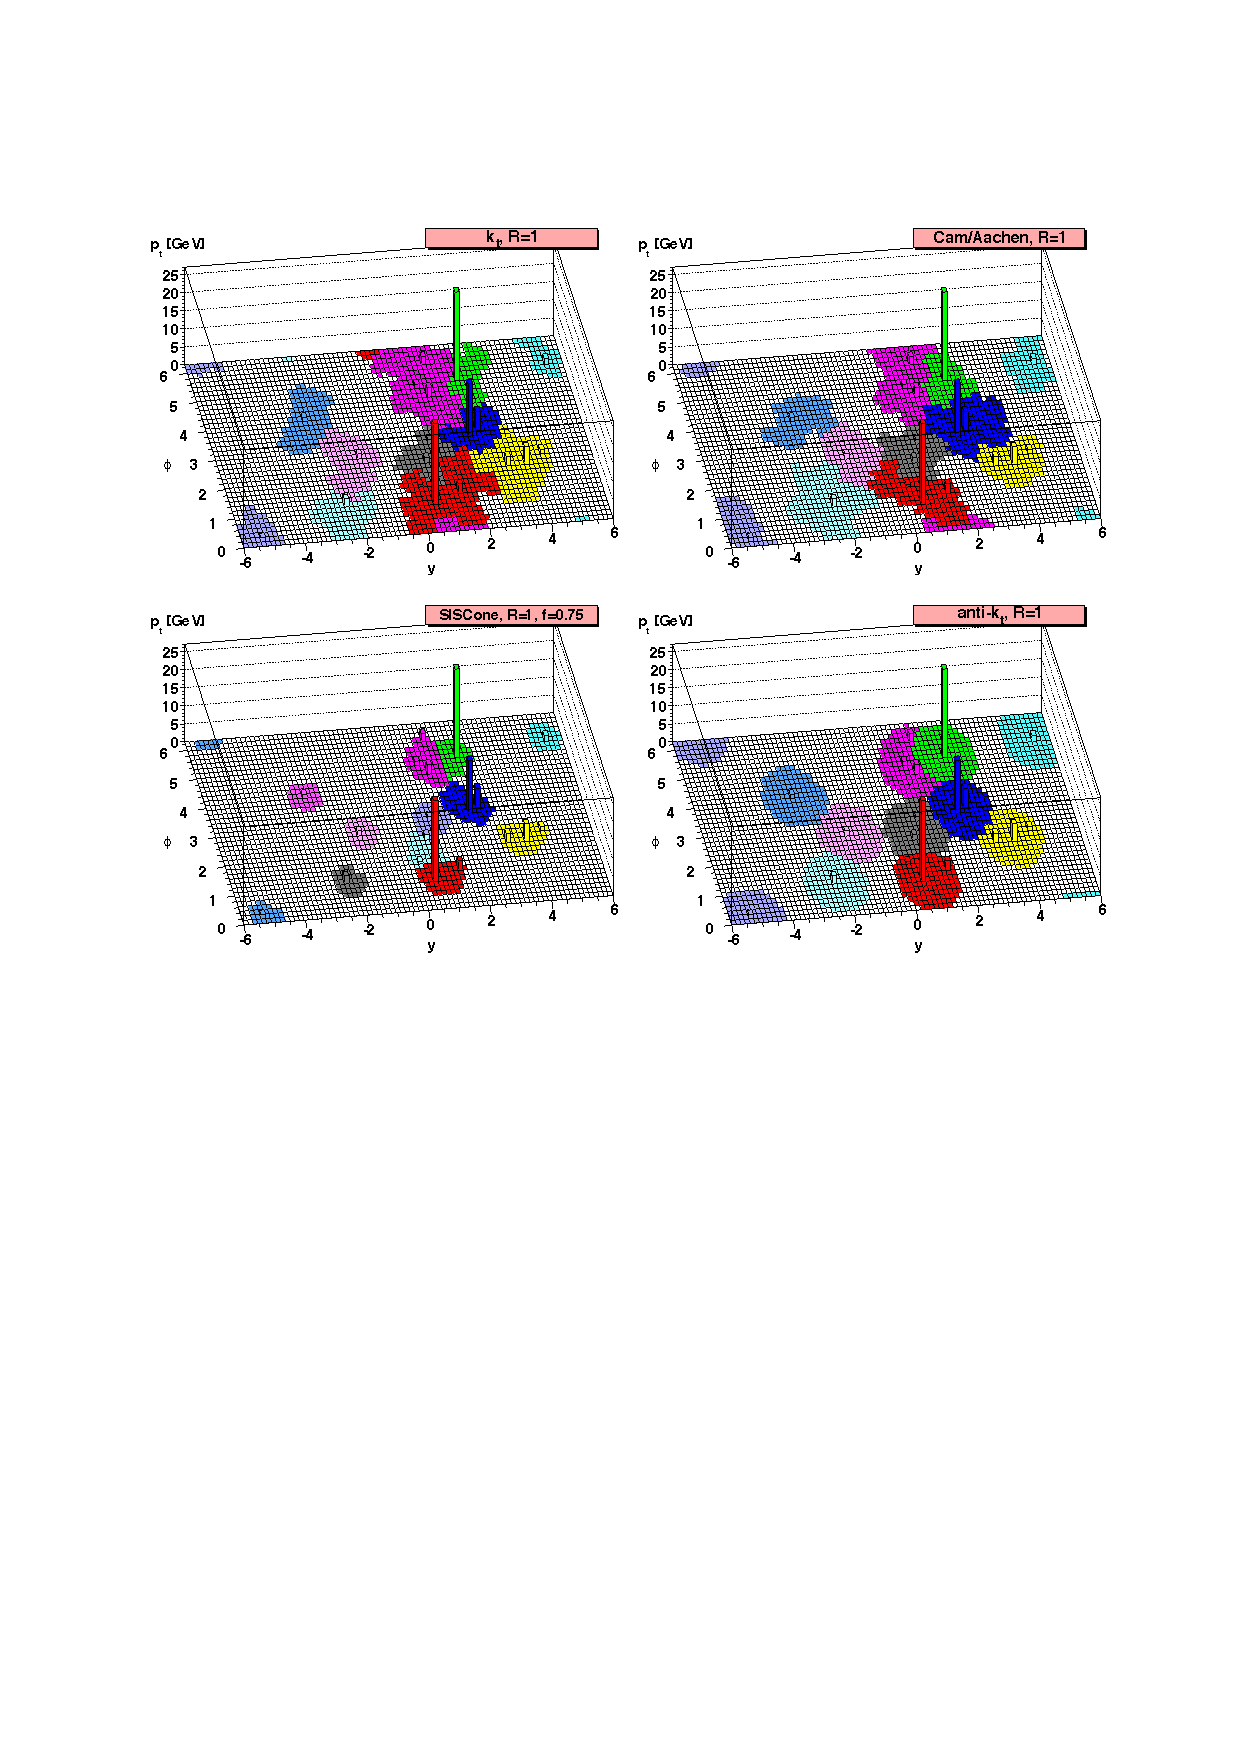
\includegraphics[width=0.9\textwidth]{Figures/diff_algos.pdf}
		%\rule{35em}{0.5pt}
	\caption[Clustering particles into jets with different algorithms.]{Clustering same set of reconstructed particles into jets using different jet algorithms. \cite{Salam:2009jx}}
	\label{fig:jetAlgos}
\end{figure}
\par Parameter $p$ defines which particles are clustered first thus defining the type of algorithm. The $k_T$ algorithm uses $p=1$, clustering soft particles first. This results in irregularly shaped jets, as shown in figure \ref{fig:jetAlgos}, which are sensitive to radiation in the event and difficult to calibrate. The \textit{Cambridge-Aachen} algorithm (CA) uses $p=0$ thus relying only on angular distribution of the input particles. This approach is particularly useful for jet substructure analysis and is less sensitive to radiation. The algorithm used in this analysis is $anti-k_T$ algorithm where $p=-1$ clusterizing the hardest particles first \cite{Cacciari:2008gp}. $Anti-k_T$ is an IRC safe algorithm with jets that are circular in shape because they are not affected by the softer components of the jet.       


%-----------------------------------
%	SUBSECTION 3.2
%-----------------------------------

\subsection{Jet corrections}
\label{sec:jetCorr}

Measured jet energy at detector level in general doesn't correspond to the energy of the originating particle. Jet calibration procedure is introduced to compensate for the nonlinear response of the calorimeters. This is done using a factorized approach where corrections on each level of correction are determined separately as described in \cite{Chatrchyan:2011ds}. Final corrected jet momentum is obtained from measured $p^{raw}$ according to:
\begin{equation}
p^{corr} = C_{offset}(p_T^{raw},\eta)\times C_{rel}(\eta) \times C_{abs}(p'_T) \times C_{res}(p_T'',\eta) \times p^{raw}
\end{equation}     
where offset correction $C_{offset}$ and calibration factors $C_{rel}$ and $C_{abs}$ are applied to both data and simulation, $C_{res}$ is applied only to data. Corrections are applied sequentially, in a fixed order such that $p_T' = C_{offset} \times C_{rel}(\eta) \times p^{raw}$ , and $p_T'' = C_{rel}(\eta) \times C_{abs}(p'_T)$. Correction factors used in this analysis can be found in \cite{CMS-DP-2013-033}.
Each level of corrections is summarized below:
\begin{itemize}
\item Offset correction $C_{offset}$ compensates for energy contributions arising from pile-up events or instrument noise. The offset is determined in dependence of pseudorapidity, jet area $p_T density$ which is described in \cite{Cacciari2008119}.
\item Relative correction $C_{rel}$ is aimed to flattening the jet scale in pseudorapidity. The correction is determined from simulation, adjusting the jet scale in all $\eta$ regions to one of the jets in $|\eta|<1.3$ without changing the absolute scale.
\item Absolute correction $C_{abs}$ flattens the jet scale in $p_T$. This correction is also determined from QCD multijet events as inverse of average response at fixed $p_T^{gen}$.
\item Residual correction $C_{res}$ is applied only to data in order to account for possible residual differences in data and simulation agreement after applying absolute and relative corrections. These corrections are derived using events with momentum balance in transverse plane, like dijet events or $Z/\gamma$ + jet events.
\end{itemize}
The total jet correction for a fixed jet $p_T$ as a function of pseudorapidity is shown in figure \ref{fig:tot_corr_eta}.
\begin{figure}[htbp]
	\centering
		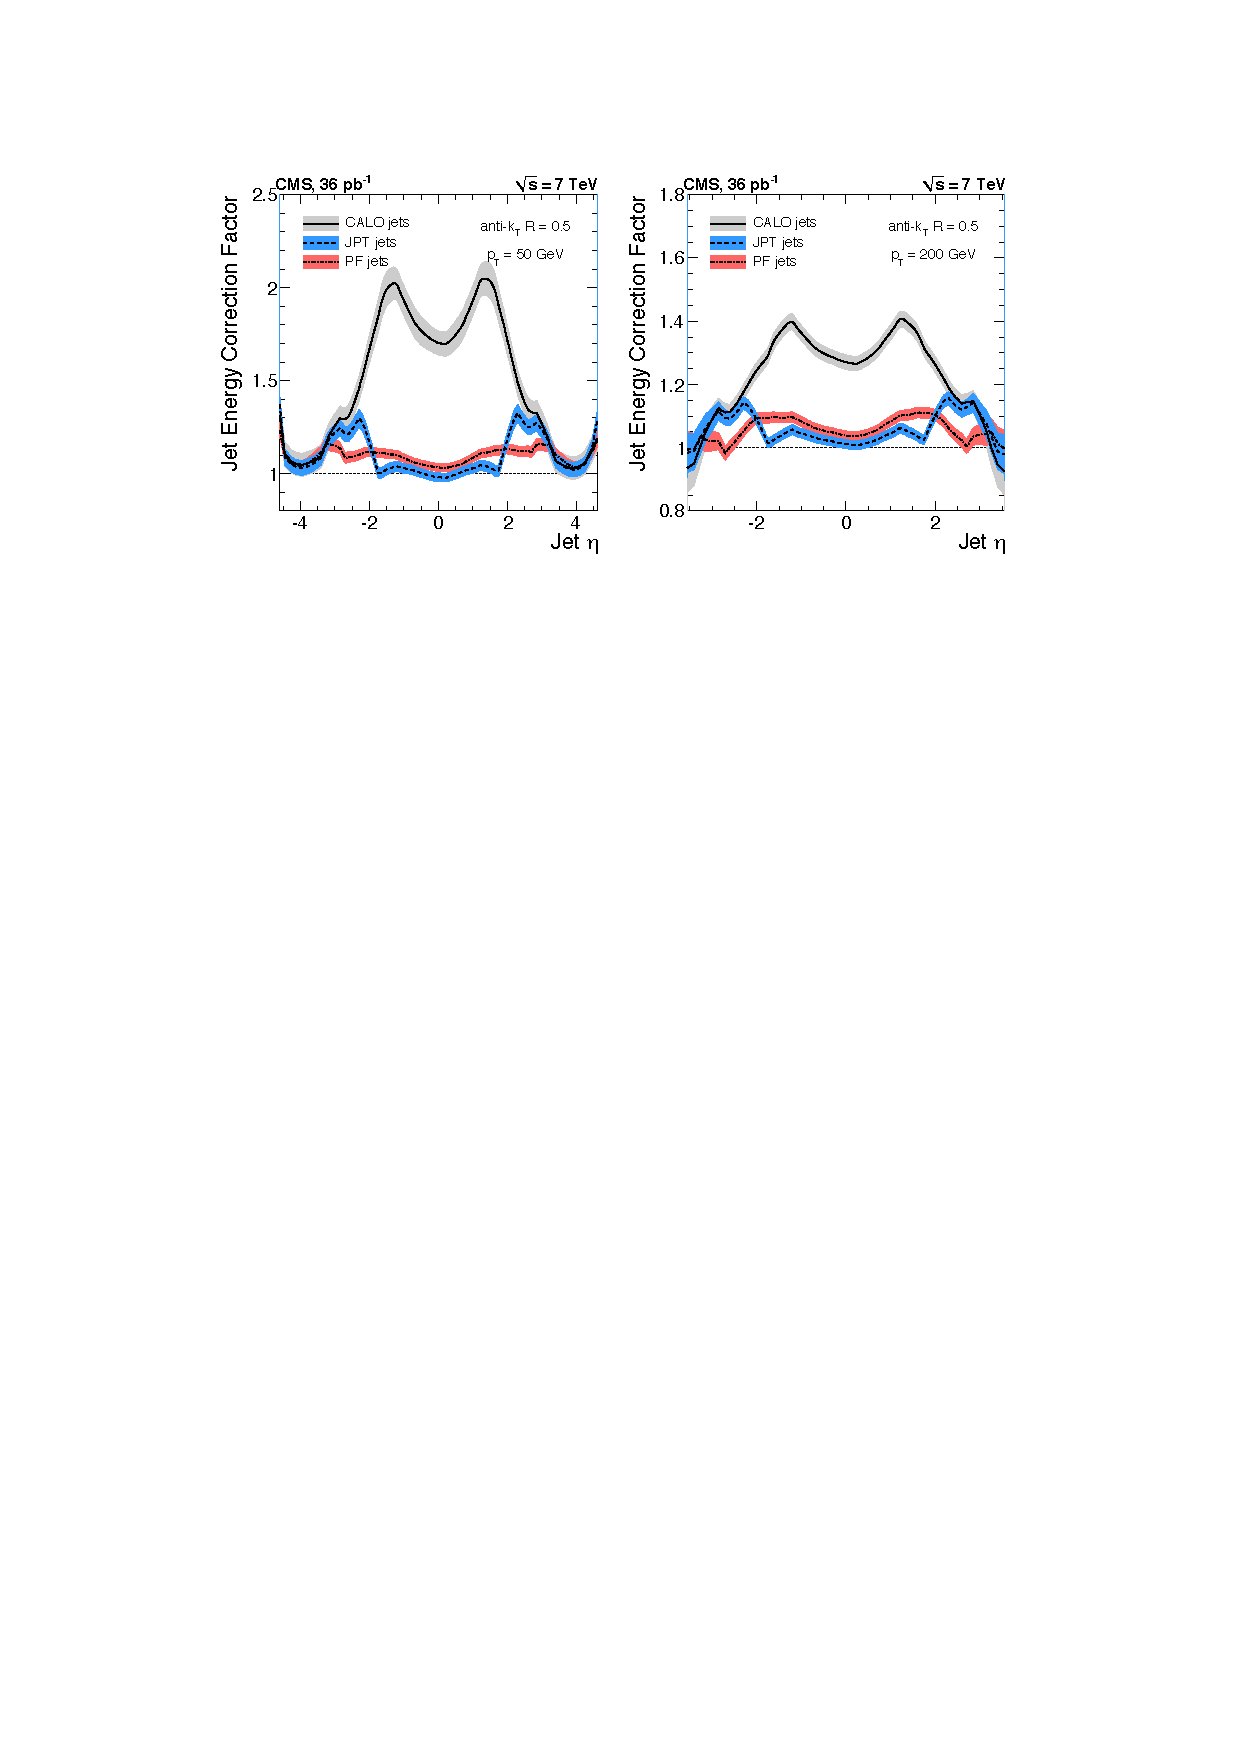
\includegraphics[width=0.9\textwidth]{Figures/jet_tot_corr_eta.pdf}
		%\rule{35em}{0.5pt}
	\caption[Total jet energy correction as a function of pseudorapidity of two different jet $p_T$ values.]{Total jet energy correction as a function of pseudorapidity of two different jet $p_T$ values. Corrections are shown for all three types of jets, calo, JPT and PF jets. Bands indicate corresponding uncertainty.}
	\label{fig:tot_corr_eta}
\end{figure}

\begin{figure}[htbp]
	\centering
		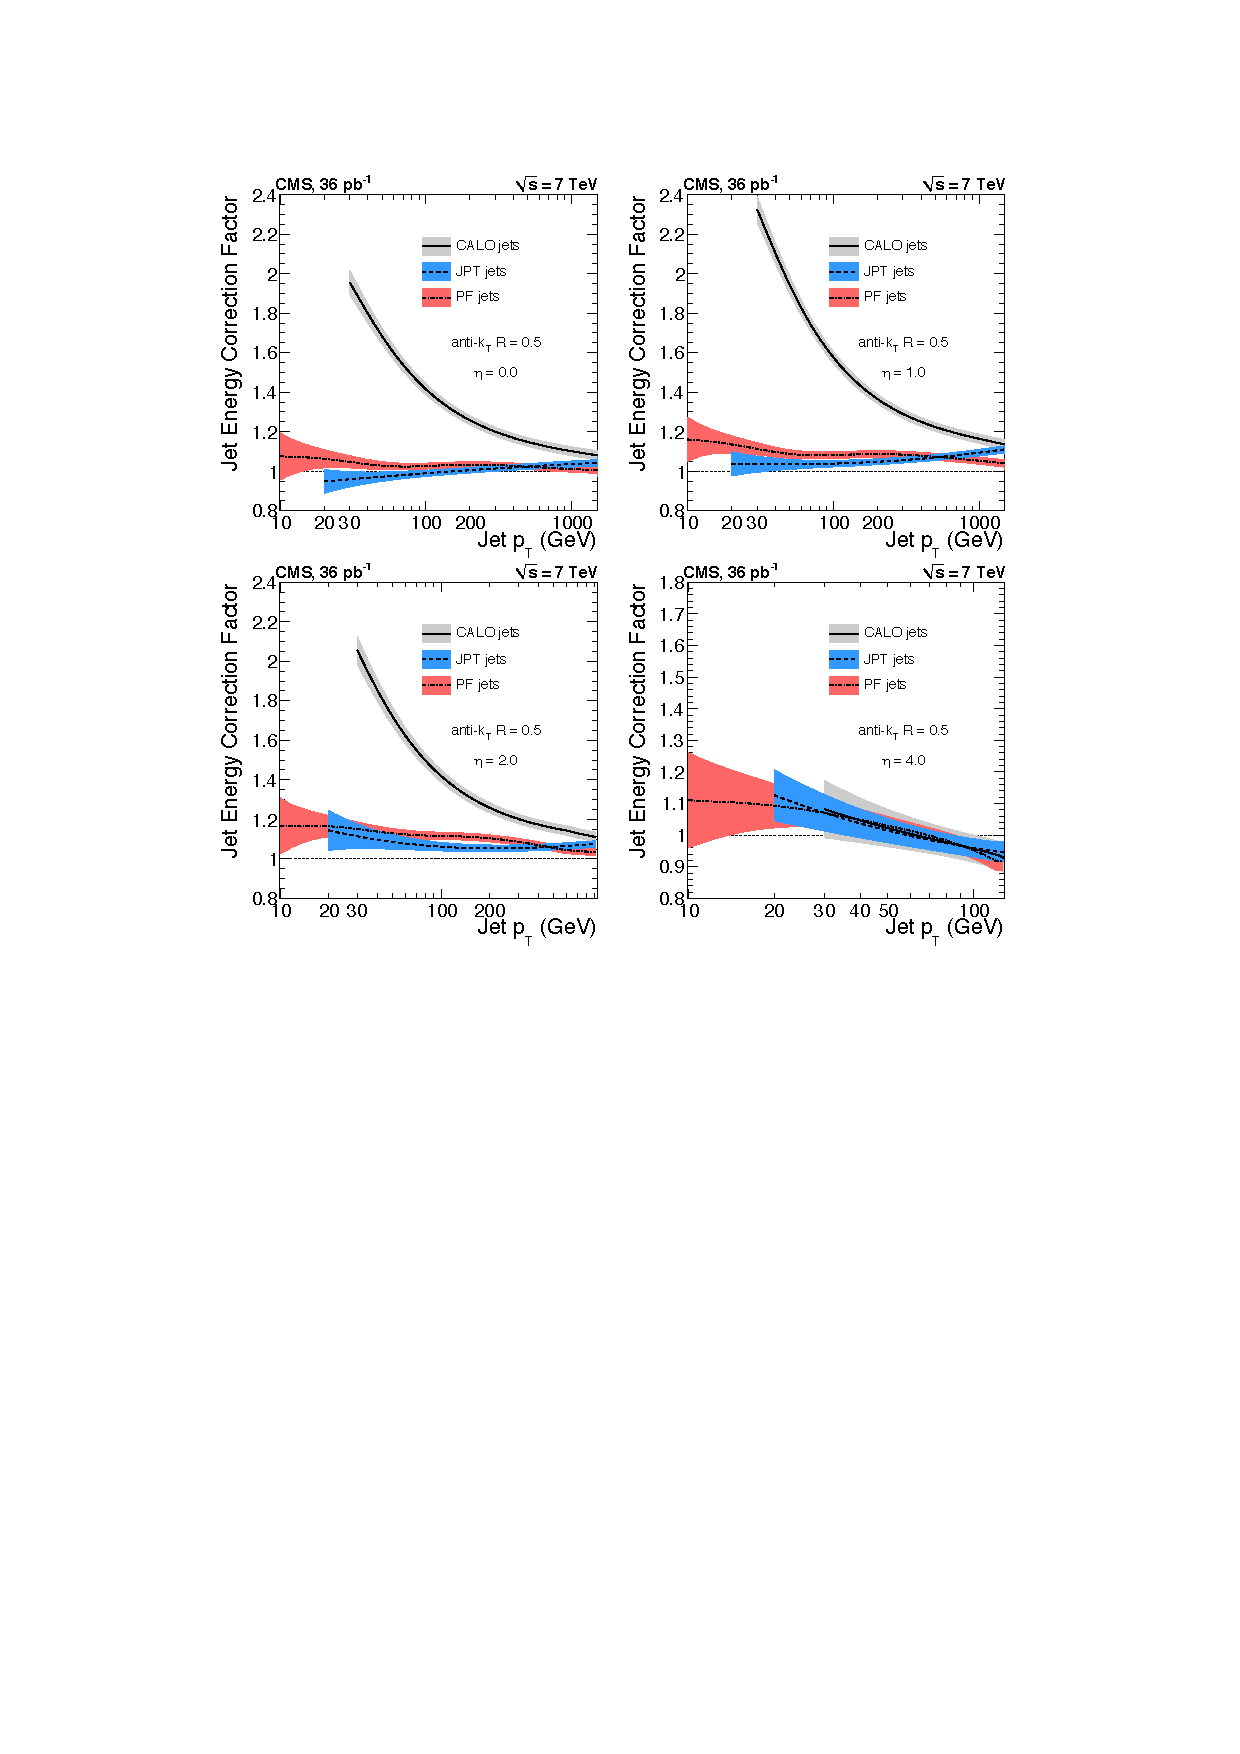
\includegraphics[width=0.9\textwidth]{Figures/jet_tot_corr_pt.pdf}
		%\rule{35em}{0.5pt}
	\caption[Total jet energy correction as a function of transverse momentum for four different $\eta$ values.]{Total jet energy correction as a function of transverse momentum for four different $\eta$ values. Corrections are shown for all three types of jets, calo, JPT and PF jets. Bands indicate corresponding uncertainty.}
	\label{fig:tot_corr_pt}
\end{figure}
%-----------------------------------
%	SUBSECTION 3.3
%-----------------------------------

\subsection{Jet identification}
\label{sec:jetID}
This analysis uses $anti-k_T$ algorithm with cone size $R=0.5$. Jet algorithm implementation is done in the \textit{Fast-jet} package \cite{Cacciari:2011ma}. Depending on which signals is the algorithm applied to, there are different kinds of jets: calo jets (using calorimeter deposits), jet-plus-track jets (calorimeter deposits complemented with tracker information) and most widely used \textit{particle flow} jets (PF). These jets are clustered from PF particles identified with PF algorithm, thus using the information not only from HCAL, but also from tracking system and ECAL which show much better resolution. Only neutral fraction of the jet is measured only with HCAL which makes about 15$\%$ of the total jet composition. PF jets show excellent performance and are the default jets for most CMS analysis. Pile-up information is also taken into account by removing charged hadrons originating from pile-up vertices from the list of particles available for the jet clusterization. This procedure is called \textit{charged hadron subtraction}. Some additional cuts to the jet composition are applied in order to endure good jet identification.  
  \begin{table}[h]
\centering
  \caption{A summary of jet identification criteria.}
  \label{tab:jetID}
  \begin{tabular}{ l  c c}
      \hline
      \hline
      	Variable & Requirement \\
      	\hline
    		Neutral hadron fraction & $<$ 0.99  \\
     	Neutral EM fraction & $<$ 0.99 \\
     	Number of Constituents & $>$ 1 \\		
		\hline
		Additional cuts for $|\eta|<2.4$ \\
		\hline
		Charged hadron fraction & $>$ 0 \\ 
		Charged multiplicity & $>$ 0 \\
		Charged EM fraction & $<$ 0.99 \\
      \hline
      \hline 
  \end{tabular}
\end{table}

%-----------------------------------
%	SUBSECTION 3.4
%-----------------------------------

\subsection{Jets from b quarks}
\label{sec:btagging}

Unique properties of the bottom quark can be used to identify hadronic jets originating from b quarks which are usually referred to as b-jets. Long lifetime of B hadrons is a consequence of weak force decay which results in their displacement by few micrometers at the LHC energies. B hadron decays show a large number of tracks with hard $p_T$ spectrum and soft leptons emerging from semi-leptonic decays. The process of b-jet identification is called $b-tagging$. This process takes one or more variables and produces a single discriminant value for each jet. This value shows how much the observed jet looks like a b-jet. There are several \textit{b-tagging} algorithms in use at CMS which are described in detail in \cite{Chatrchyan:2012jua} and the following were used in 2012 data analysis:
\begin{itemize}
	\item \textit{Track counting}(TC) - The discriminant value is the impact parameter significance which is calculated as impact parameter value divided by the respective impact parameter uncertainty. Impact parameter values are sorted in the decreasing order. Depending on whether second or third value is chosen, the algorithm is denoted as high efficiency or high purity. 
	\item \textit{Jet Probability}(JP) - This algorithm combines information from several tracks inside a jet by computing a likelihood thet all tracks originated from the primary vertex.  
	\item \textit{Combined secondary vertex}(CSV) - This is the most efficient \textit{b-tagging} algorithm currently used at CMS. Both secondary vertex and track related information are combined to build a CSV discriminant value. It shows high efficiency even when no good secondary vertex can be reconstructed. Some of the variables used in CSV algorithm are flight distance, vertex mass, impact parameter significance, track multiplicity at the vertex and track multiplicity in a jet. The distribution of CSV discriminant value is shown in figure \ref{fig:csv}.
\end{itemize}
\begin{figure}[ht]
	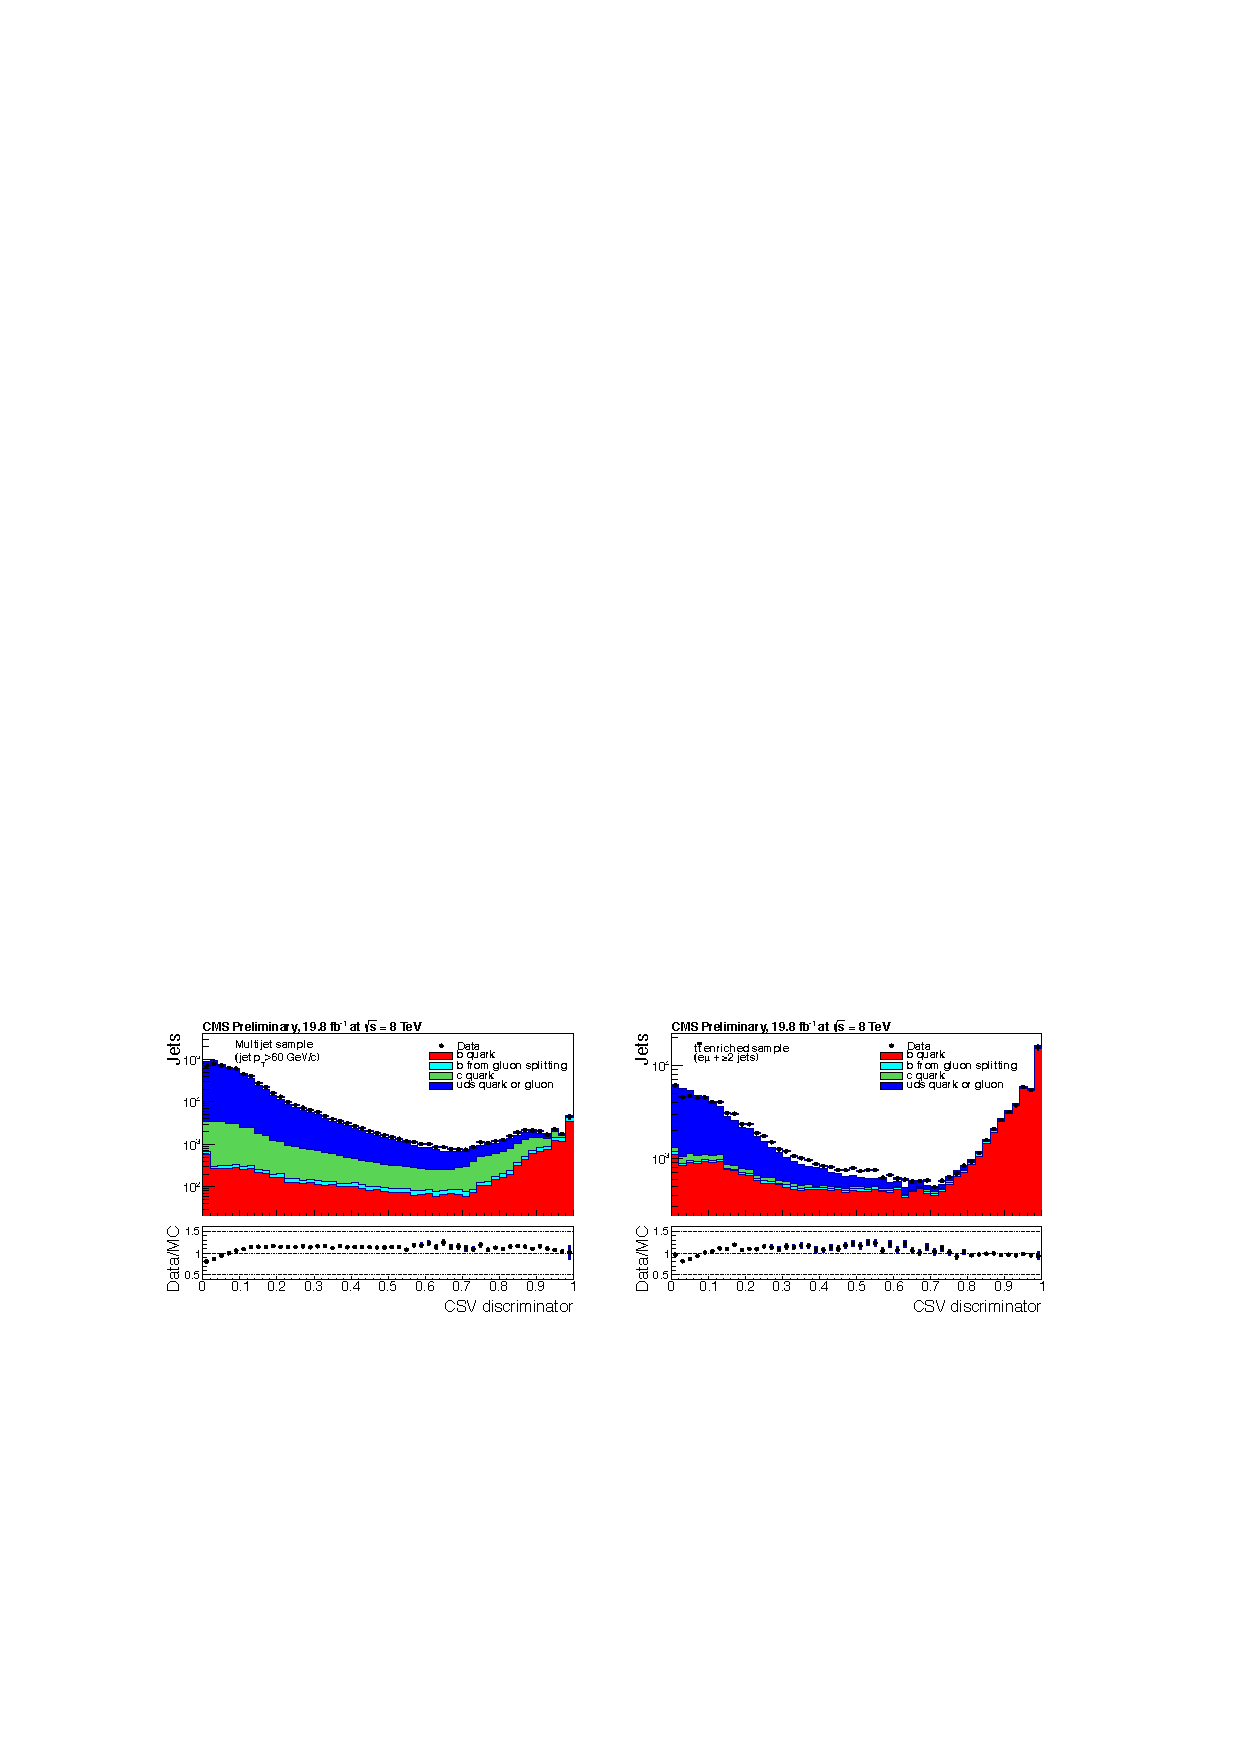
\includegraphics[width=\textwidth]{Figures/b-tag_csv.pdf}
	\caption{Combined secondary vertex discriminant value for multijet QCD sample (left) and tt enriched sample(right)\cite{CMS:2013vea}}
	\label{fig:csv}
\end{figure}
For each non-b-jet there is a chance that it would be identified as b-jet. Based on this misidentification rate, three operating points have been defined for the discriminant value: loose, medium and tight. For an average jet of 80 GeV, these values correspond to misidentification rates of 10\%, 1\% and 0.1\% respectively. Misidentification probabilities as a function of b-jer efficiency for several algorithms are shown in figure \ref{fig:misID}. 
\begin{figure}[ht]
\centering
	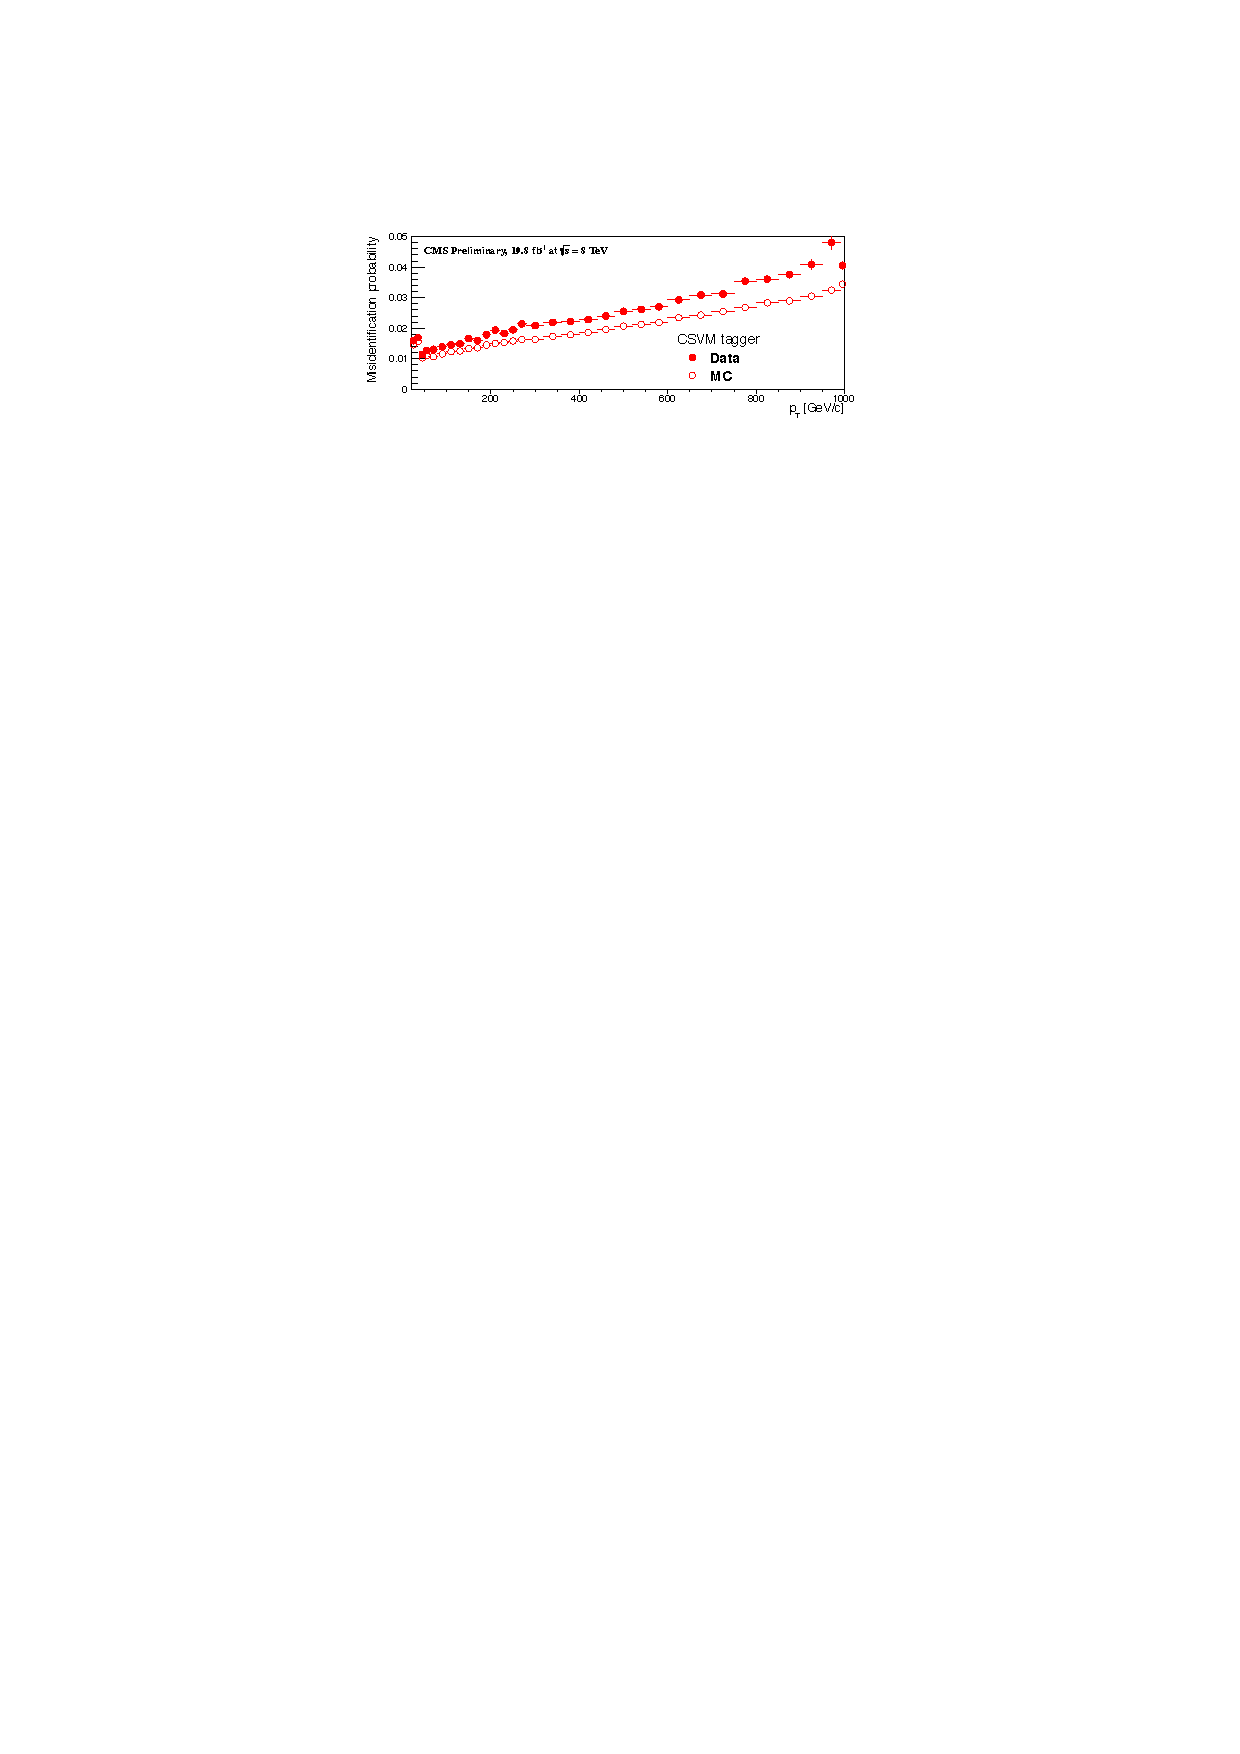
\includegraphics[width=0.6\textwidth]{Figures/MisID_CSVM.pdf}
	\caption{Combined secondary vertex misidentification probability for data and MC for medium working point.\cite{CMS:2013vea}}
	\label{fig:misID}
\end{figure}



%----------------------------------------------------------------------------------------
%	SECTION 4
%----------------------------------------------------------------------------------------

\section{Missing transverse energy}

Missing transverse momentum is the imbalance in the vectorial sum of transverse momenta of all measured particles. Momentum conservation delegates that the imbalance arises from weakly interacting neutral particles such as neutrinos. Missing transverse energy is the magnitude of the missing transverse momentum and is calculated as:
\begin{equation}
E_T^{miss}= |-\sum_{i} \vec{p}_i|
\end{equation}
where $i$ goes over all visible particles. Measurement of the missing transverse energy relies on the good measurement of all other particles in the event and as such is very sensitive to detector inefficiencies, particle missmeasurements, limited acceptance of the detector, cosmic-ray particles all of which can cause artificial missing energy. There are several approaches to determine $E_T^{miss}$. In this analysis, particle flow technique is used which tries to identify each particle in the event by combining the information from all subdetectors and gives the best missing energy resolution.\cite{CMS-PAS-PFT-09-001,Chatrchyan:2011tn} Several corrections are applied to the $E_T^{miss}$ which correct for the possible bias in the missing energy measurement:
\begin{itemize}
\item Type-I correction: propagates jet energy corrections described in Section \ref{sec:jetCorr} to missing energy. This correction replaces the missing energy calculated by summing transverse momenta of particles in a jet by transverse momentum of a jet to which JEC were applied.
\item xy-shift correction: aimed at correcting the observed missing energy $\phi$ modulation. True missing energy distribution is expected not to depend not to depend of $\phi$ because of the rotational symmetry of collisions around the beam axis. The possible cause for such modulation  include unisotropic detector response, detector misalignment, the displacement of the beam spot. The amplitude of the modulation is observed to increase with the number of pile-up interactions so this correction can be seen as mitigation for the pile-up effects.
\end{itemize}




 
% Chapter Template

\chapter{Event selection and analysis strategy} % Main chapter title

\label{Chapter6} % Change X to a consecutive number; for referencing this chapter elsewhere, use \ref{ChapterX}

\lhead{Chapter 6. \emph{Event selection and analysis strategy}} % Change X to a consecutive number; this is for the header on each page - perhaps a shortened title

%----------------------------------------------------------------------------------------
%	SECTION 1
%----------------------------------------------------------------------------------------

\section{Analysis strategy}


%-----------------------------------
%	SUBSECTION 1
%-----------------------------------
\subsection{Subsection 1}



%-----------------------------------
%	SUBSECTION 2
%-----------------------------------

\subsection{Subsection 2}


%----------------------------------------------------------------------------------------
%	SECTION 2
%----------------------------------------------------------------------------------------

\section{Background estimation}

 
%% Chapter Template

\chapter{Prosireni sazetak:} % Main chapter title

\label{Chapter7} % Change X to a consecutive number; for referencing this chapter elsewhere, use \ref{ChapterX}

\lhead{Chapter X. \emph{Chapter Title Here}} % Change X to a consecutive number; this is for the header on each page - perhaps a shortened title

%----------------------------------------------------------------------------------------
%	SECTION 1
%----------------------------------------------------------------------------------------

\section{Main Section 1}

Lorem ipsum dolor sit amet, consectetur adipiscing elit. Aliquam ultricies lacinia euismod. Nam tempus risus in dolor rhoncus in interdum enim tincidunt. Donec vel nunc neque. In condimentum ullamcorper quam non consequat. Fusce sagittis tempor feugiat. Fusce magna erat, molestie eu convallis ut, tempus sed arcu. Quisque molestie, ante a tincidunt ullamcorper, sapien enim dignissim lacus, in semper nibh erat lobortis purus. Integer dapibus ligula ac risus convallis pellentesque.

%-----------------------------------
%	SUBSECTION 1
%-----------------------------------
\subsection{Subsection 1}

Nunc posuere quam at lectus tristique eu ultrices augue venenatis. Vestibulum ante ipsum primis in faucibus orci luctus et ultrices posuere cubilia Curae; Aliquam erat volutpat. Vivamus sodales tortor eget quam adipiscing in vulputate ante ullamcorper. Sed eros ante, lacinia et sollicitudin et, aliquam sit amet augue. In hac habitasse platea dictumst.

%-----------------------------------
%	SUBSECTION 2
%-----------------------------------

\subsection{Subsection 2}
Morbi rutrum odio eget arcu adipiscing sodales. Aenean et purus a est pulvinar pellentesque. Cras in elit neque, quis varius elit. Phasellus fringilla, nibh eu tempus venenatis, dolor elit posuere quam, quis adipiscing urna leo nec orci. Sed nec nulla auctor odio aliquet consequat. Ut nec nulla in ante ullamcorper aliquam at sed dolor. Phasellus fermentum magna in augue gravida cursus. Cras sed pretium lorem. Pellentesque eget ornare odio. Proin accumsan, massa viverra cursus pharetra, ipsum nisi lobortis velit, a malesuada dolor lorem eu neque.

%----------------------------------------------------------------------------------------
%	SECTION 2
%----------------------------------------------------------------------------------------

\section{Main Section 2}

Sed ullamcorper quam eu nisl interdum at interdum enim egestas. Aliquam placerat justo sed lectus lobortis ut porta nisl porttitor. Vestibulum mi dolor, lacinia molestie gravida at, tempus vitae ligula. Donec eget quam sapien, in viverra eros. Donec pellentesque justo a massa fringilla non vestibulum metus vestibulum. Vestibulum in orci quis felis tempor lacinia. Vivamus ornare ultrices facilisis. Ut hendrerit volutpat vulputate. Morbi condimentum venenatis augue, id porta ipsum vulputate in. Curabitur luctus tempus justo. Vestibulum risus lectus, adipiscing nec condimentum quis, condimentum nec nisl. Aliquam dictum sagittis velit sed iaculis. Morbi tristique augue sit amet nulla pulvinar id facilisis ligula mollis. Nam elit libero, tincidunt ut aliquam at, molestie in quam. Aenean rhoncus vehicula hendrerit. 

%----------------------------------------------------------------------------------------
%	THESIS CONTENT - APPENDICES
%----------------------------------------------------------------------------------------

\addtocontents{toc}{\vspace{2em}} % Add a gap in the Contents, for aesthetics

\appendix % Cue to tell LaTeX that the following 'chapters' are Appendices

% Include the appendices of the thesis as separate files from the Appendices folder
% Uncomment the lines as you write the Appendices

% Appendix A

\chapter{Lorentz angle measurement in Pixel detector} % Main appendix title

\label{AppendixA} % For referencing this appendix elsewhere, use \ref{AppendixA}

\lhead{Appendix A. \emph{Lorentz angle measurement in Pixel detector}} 

\section{Grazing angle method}
Lorentz angle is measured by using grazing angle method described in detail in \cite{Henrich}. From the individual signals in the detector, using reconstruction algorithms, tracks of muon candidates are obtained. From these reconstructed track it is possible to extract the entry point ($x_{reco}$,$y_{reco}$) to each layer of the detector. 
Distance between reconstructed entry point and the actual hit in the detector is then defined as ($\Delta x$,$\Delta y$):
\begin{equation}
\Delta x = x_{center}-x_{reco}
\end{equation} 
\begin{equation}
\Delta y = y_{center}-y_{reco}
\end{equation} 

where ($x_{center}$,$y_{center}$) is the position of each individual pixel center in the observed cluster. Drift of the electrons can be determined using three impact angles defined in the following way:

\begin{equation}
\text{tan} \alpha = \frac{p_z}{p_x}
\end{equation}
\begin{equation}
\text{tan} \beta = \frac{p_z}{p_y}
\end{equation}
\begin{equation}
\text{tan} \gamma = \frac{p_x}{p_y}
\end{equation}

where $p_x$,$p_y$ and $p_z$ are momentum components in local coordinate system which are calculated from reconstructed track parameters (Fig. \ref{fig:kut}). \\
\begin{figure}[ht!]
\centering
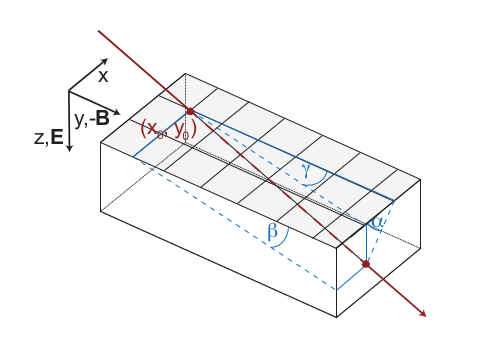
\includegraphics[width=0.5\textwidth]{Figures/kut.png}
\caption{Angle definitions for grazing angle method.}
\label{fig:kut}
\end{figure}
Drift of the electrons depends on the depth at which electrons are created. Depth of the electron production $z$ and drift due to magnetic field $d$ are defined:

\begin{equation}
z = \Delta y \text{ tan}\beta
\end{equation}
\begin{equation}
d=\Delta x-\Delta y \text{ tan}\gamma
\end{equation}

This procedure is repeated for each pixel over many tracks in order to obtain charge drift distance vs depth. The Lorentz angle is the slope of this distribution.  Without a magnetic field, the
direction of the clusters largest extension is parallel to the track projection on the (x, y) plane. The average drift distance of an electron created at a certain depth is obtained from Fig. \ref{fig:2D}. A linear fit is
performed over the total depth of the detector excluding the first and last 50 $\mu$ where the charge drift is systematically displaced by the finite size of the pixel cell (Fig:\ref{fig:profile}). 

\begin{figure}[ht!]
\centering
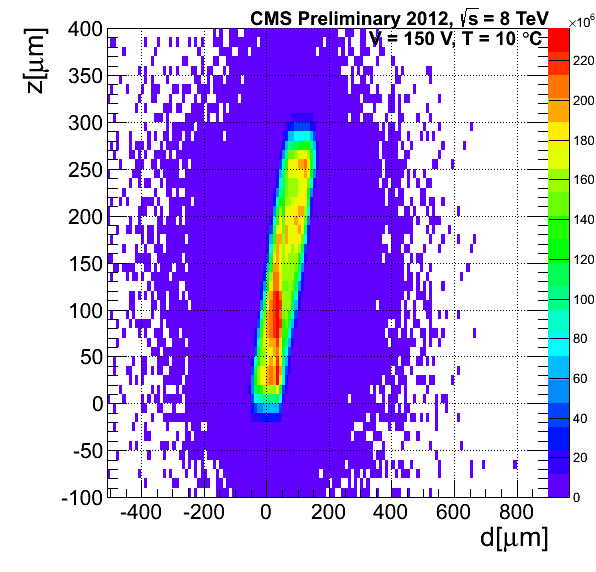
\includegraphics[width=0.5\textwidth]{Figures/LA2012_2D.png}
\caption{Depth at which electrons in silicon bulk were produced as a function of Lorentz drift.}
\label{fig:2D}
\end{figure}

\begin{figure}[ht!]
\centering
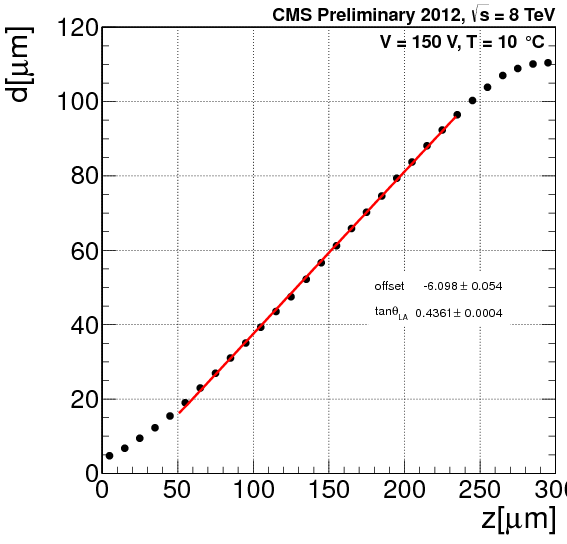
\includegraphics[width=0.5\textwidth]{Figures/LA2012_Profile.png}
\caption{The average drift of electrons as a function of the production depth. Slope of the linear fit result is the $tan \theta_L$.}
\label{fig:profile}
\end{figure}

In order to obtain a good measurement, it is important to use clean tracks. Therefore, it required to have a well reconstructed muon tracks with $p_T>3$GeV and $\chi^2/ndof<2$ which are required to have shallow impact angle with respect to local $y$ direction with cluster size of at least 4 pixels in this direction. Summary of the selection criteria can be found in table \ref{tab:sel}.

\begin{table}[ht!]
  \caption{Selection criteria for Lorentz angle measurement}
  \centering
  \begin{tabular}{l|c}
\hline
\hline
        Cluster size in y & $>3$  \\
	Track $p_t$ & $>3$GeV$/$c \\
	$\chi^2$/ndof & $<2$ \\
	Hit residuals & $<50\mu m$ \\
	Cluster charge & $<120000$e \\
\hline
\hline
  \end{tabular}
  \label{tab:sel}
\end{table}

Figure \ref{fig:La2012} shows how Lorentz angle changes with integrated luminosity. Results are shown for 23fb$^{-1}$ of delivered luminosity in 2012. Increase in Lorentz angle measured with grazing angle method has been observed in all layers, with largest effect (~6\%) visible in layer 1 over this period of data taking.  
\begin{figure}[ht!]
\centering
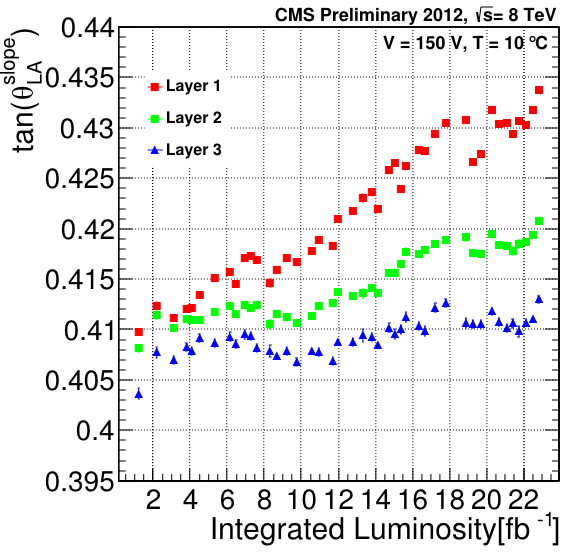
\includegraphics[width=0.5\textwidth]{Figures/LA2012.png}
\caption{Lorentz angle as a function of integrated luminosity for 2012.}
\label{fig:La2012}
\end{figure}

\section{Minimum cluster size method (V-method)}
The pixel cluster size in the drift direction depends on the incident
angle and is minimal when incident angle is equal to the Lorentz angle. Thus, measuring the average cluster size in drift direction as a function of incident angle and obtaining a minimum of that
distribution is an alternative and direct method of measuring the Lorentz angle. The method is usually referred to as V-method due
to a shape of distribution which in the simple case can be approximated with formula

\begin{equation}
p_1*abs(tan(\theta) - p_0) + p_2
\end{equation}
where $p_0$, $p_1$ and $p_2$ are parameters obtained from the fit and $p_0$ = $tan(\theta_{LA})$.

The method was successfully applied to cosmic muon tracks during CMS commissioning period in 2008 and again in 2015. The fit result is shown in figure \ref{fig:LA_VMethod}.

\begin{figure}[hbtp!]
	\centering
	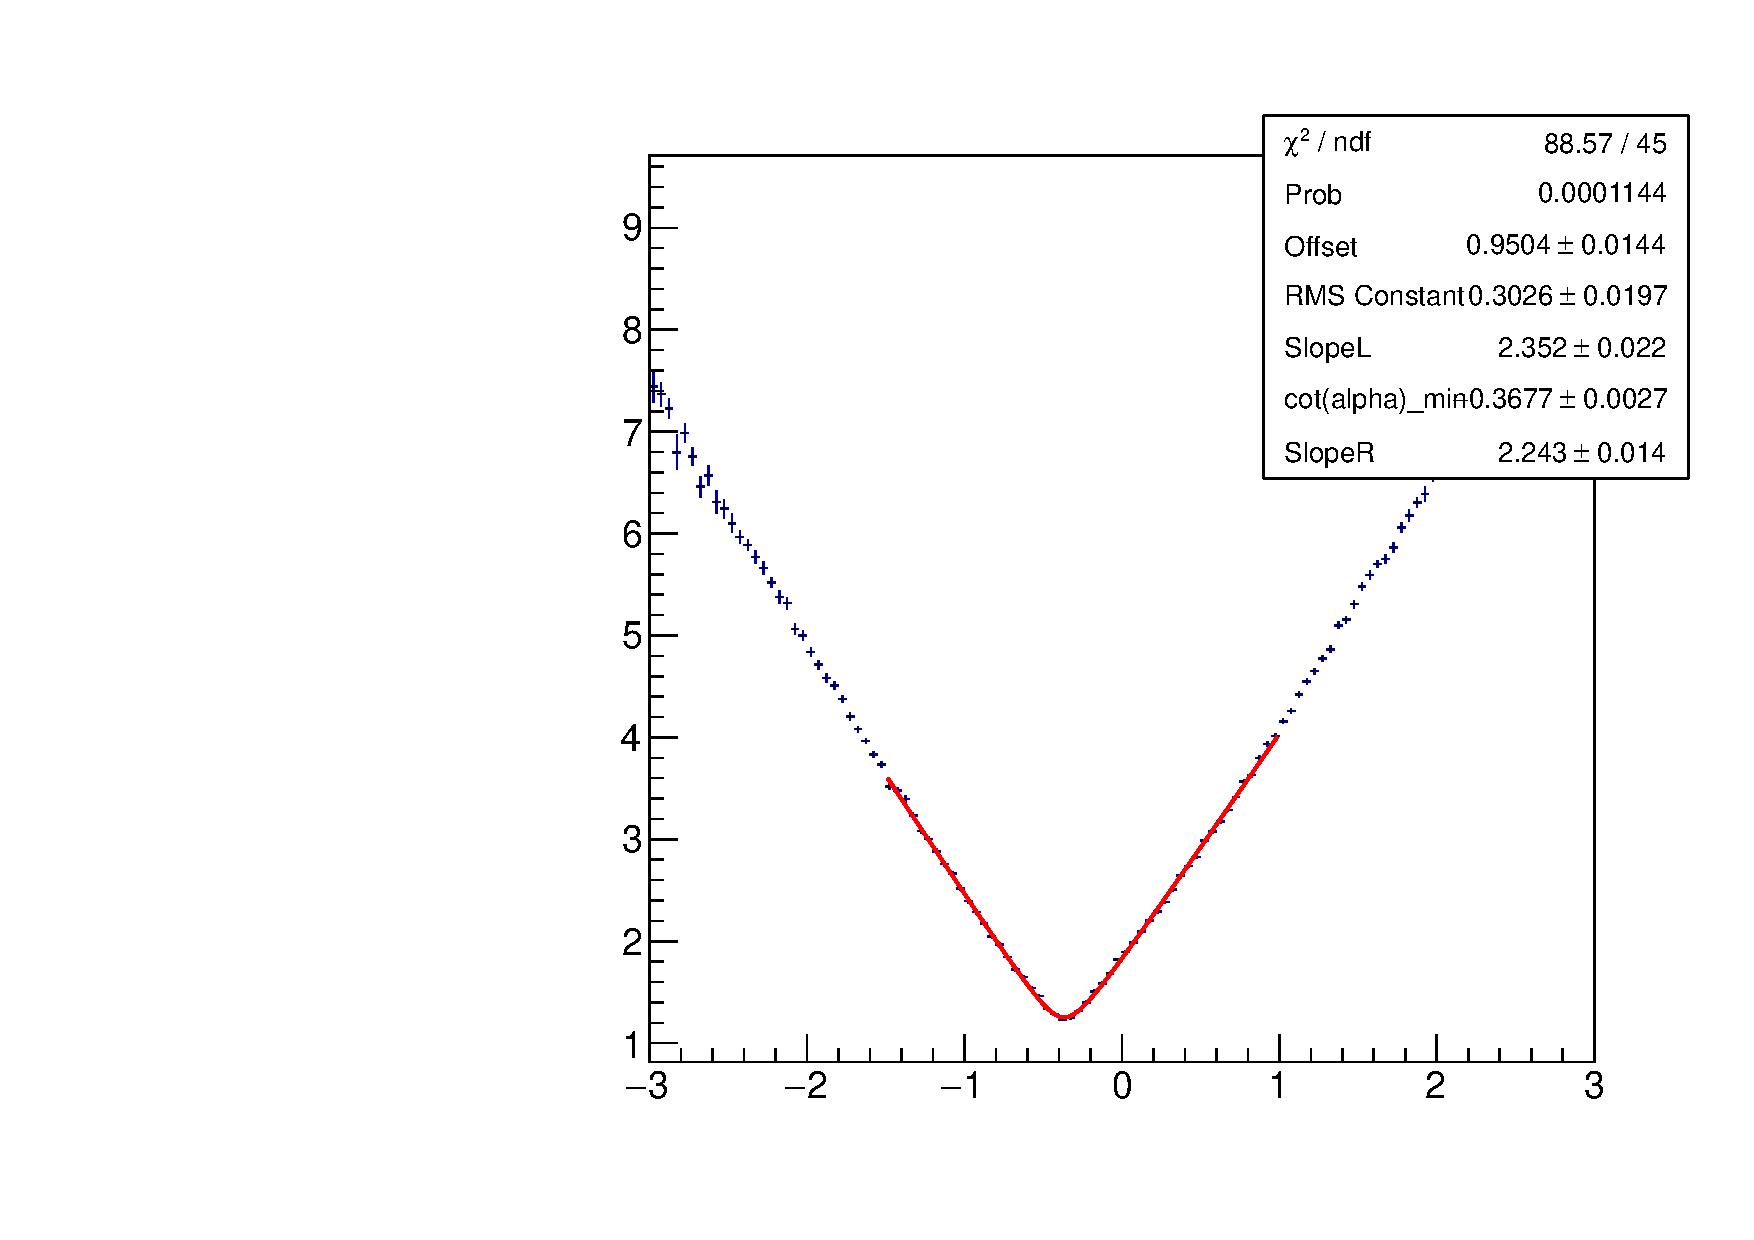
\includegraphics[width=0.5\textwidth]{Figures/LA_VMethod_2015.pdf}
\end{figure}

Application to collision data is more challenging. Coordinates of a track passing through the detector, its incoming angle, and its $p_T$ are
correlated and therefore incoming angles from collision tracks have limited range. With
standard running conditions the value of Lorentz angle is at the edge of that range where tracks with very low $p_T$ (<0.5 GeV) dominate. Because
of that average cluster size as a function of incoming angle cannot be described by a simple model like above mentioned for cosmic data.
While  results for collision data obtained with V-method are in general agreement with the default calculation,  the uncertainty of
the method at present is too big to be used as a viable alternative.


%% Appendix Template

\chapter{Acceptance and efficiency error calculation} % Main appendix title

\label{AppendixB} % Change X to a consecutive letter; for referencing this appendix elsewhere, use \ref{AppendixX}

\lhead{Appendix B. \emph{Acceptance and efficiency error calculation}} % Change X to a consecutive letter; this is for the header on each page - perhaps a shortened title

Write your Appendix content here.
%\input{Appendices/AppendixC}

\addtocontents{toc}{\vspace{2em}} % Add a gap in the Contents, for aesthetics

\backmatter

%----------------------------------------------------------------------------------------
%	BIBLIOGRAPHY
%----------------------------------------------------------------------------------------

\label{Bibliography}

\lhead{\emph{Bibliography}} % Change the page header to say "Bibliography"

%\bibliographystyle{unsrtnat} % Use the "unsrtnat" BibTeX style for formatting the Bibliography
\bibliographystyle{unsrt}

\bibliography{Bibliography}




\end{document}
